%  LaTeX support: latex@mdpi.com 
%  For support, please attach all files needed for compiling as well as the log file, and specify your operating system, LaTeX version, and LaTeX editor.

%=================================================================
\documentclass[mca,article,submit,pdftex,moreauthors]{Definitions/mdpi} 
%\documentclass[preprints,article,submit,pdftex,moreauthors]{Definitions/mdpi} 
% For posting an early version of this manuscript as a preprint, you may use "preprints" as the journal. Changing "submit" to "accept" before posting will remove line numbers.

% Below journals will use APA reference format:
% admsci, aieduc, behavsci, businesses, econometrics, economies, education, ejihpe, famsci, games, humans, ijcs, ijfs, jintelligence, journalmedia, jrfm, jsam, languages, peacestud, psycholint, publications, tourismhosp, youth

% Below journals will use Chicago reference format:
% arts, genealogy, histories, humanities, laws, literature, religions, risks, socsci

%--------------------
% Class Options:
%--------------------
%----------
% journal
%----------
% Choose between the following MDPI journals:
% accountaudit, acoustics, actuators, addictions, adhesives, admsci, adolescents, aerobiology, aerospace, agriculture, agriengineering, agrochemicals, agronomy, ai, aichem, aieduc, aieng, aimater, aimed, aipa, air, aisens, algorithms, allergies, alloys, amh, analog, analytica, analytics, anatomia, anesthres, animals, antibiotics, antibodies, antioxidants, applbiosci, appliedchem, appliedmath, appliedphys, applmech, applmicrobiol, applnano, applsci, aquacj, architecture, arm, arthropoda, arts, asc, asi, astronautics, astronomy, atmosphere, atoms, audiolres, automation, axioms, bacteria, batteries, bdcc, behavsci, beverages, biochem, bioengineering, biologics, biology, biomass, biomechanics, biomed, biomedicines, biomedinformatics, biomimetics, biomolecules, biophysica, bioresourbioprod, biosensors, biosphere, biotech, birds, blockchains, bloods, blsf, brainsci, breath, buildings, businesses, cancers, carbon, cardio, cardiogenetics, cardiovascmed, catalysts, cells, ceramics, challenges, chemengineering, chemistry, chemosensors, chemproc, children, chips, cimb, civileng, cleantechnol, climate, clinbioenerg, clinpract, clockssleep, cmd, cmtr, coasts, coatings, colloids, colorants, commodities, complexities, complications, compounds, computation, computers, condensedmatter, conservation, constrmater, cosmetics, covid, crops, cryo, cryptography, crystals, csmf, ctn, culture, curroncol, cyber, dairy, data, ddc, dentistry, dermato, dermatopathology, designs, devices, dhi, diabetology, diagnostics, dietetics, digital, disabilities, diseases, diversity, dna, drones, dynamics, earth, ebj, ecm, ecologies, econometrics, economies, edm, education, eesp, ejihpe, electricity, electrochem, electronicmat, electronics, encyclopedia, endocrines, energies, eng, engproc, entomology, entropy, environments, environremediat, epidemiologia, epigenomes, esa, est, famsci, fermentation, fibers, fintech, fire, fishes, fluids, foods, forecasting, forensicsci, forests, fossstud, foundations, fractalfract, fuels, future, futureinternet, futurepharmacol, futurephys, futuretransp, galaxies, games, gases, gastroent, gastrointestdisord, gastronomy, gels, genealogy, genes, geographies, geohazards, geomatics, geometry, geosciences, geotechnics, geriatrics, germs, glacies, grasses, green, greenhealth, gucdd, hardware, hazardousmatters, healthcare, hearts, hemato, hematolrep, hep, heritage, higheredu, highthroughput, histories, horticulturae, hospitals, humanities, humans, hydrobiology, hydrogen, hydrology, hydropower, hygiene, idr, iic, ijcs, ijem, ijerph, ijfs, ijgi, ijmd, ijms, ijns, ijom, ijpb, ijt, ijtm, ijtpp, ime, immuno, informatics, information, infrastructures, inorganics, insects, instruments, inventions, iot, j, jaestheticmed, jal, jcdd, jcm, jcp, jcrm, jcs, jcto, jdad, jdb, jdream, jemr, jeta, jfb, jfmk, jgbg, jgg, jimaging, jintelligence, jlpea, jmahp, jmmp, jmms, jmp, jmse, jne, jnt, jof, joi, joitmc, joma, jop, joptm, jor, journalmedia, jox, jpbi, jphytomed, jpm, jrfm, jsam, jsan, jtaer, jvd, jzbg, kidneydial, kinasesphosphatases, knowledge, labmed, laboratories, lae, land, languages, laws, life, lights, limnolrev, lipidology, liquids, literature, livers, logics, logistics, lubricants, lymphatics, machines, macromol, magnetism, magnetochemistry, make, marinedrugs, materials, materproc, mathematics, mca, measurements, medicina, medicines, medsci, membranes, merits, metabolites, metals, meteorology, methane, metrics, metrology, micro, microarrays, microbiolres, microelectronics, micromachines, microorganisms, microplastics, microwave, minerals, mining, mmphys, modelling, molbank, molecules, mps, msf, mti, multimedia, muscles, nanoenergyadv, nanomanufacturing, nanomaterials, ncrna, ndt, network, neuroglia, neuroimaging, neurolint, neurosci, nitrogen, notspecified, nursrep, nutraceuticals, nutrients, obesities, occuphealth, oceans, ohbm, onco, optics, oral, organics, organoids, osteology, oxygen, pandemics, parasites, parasitologia, particles, pathogens, pathophysiology, peacestud, pediatrrep, pets, pharmaceuticals, pharmaceutics, pharmacoepidemiology, pharmacy, philosophies, photochem, photonics, phycology, physchem, physics, physiologia, plants, plasma, platforms, pollutants, polymers, polysaccharides, populations, poultry, powders, precipitation, precisoncol, preprints, proceedings, processes, prosthesis, proteomes, psf, psychiatryint, psychoactives, psycholint, publications, purification, quantumrep, quaternary, qubs, radiation, rdt, reactions, realestate, receptors, recycling, regeneration, religions, remotesensing, reports, reprodmed, resources, rheumato, risks, rjpm, robotics, rsee, ruminants, safety, sci, scipharm, sclerosis, seeds, sensors, separations, sexes, shi, signals, sinusitis, siuj, skins, smartcities, sna, societies, socsci, software, soilsystems, solar, solids, spectroscj, sports, standards, stats, std, stratsediment, stresses, surfaces, surgeries, suschem, sustainability, symmetry, synbio, systems, tae, targets, taxonomy, technologies, telecom, test, textiles, thalassrep, therapeutics, thermo, timespace, tomography, tourismhosp, toxics, toxins, tph, transplantology, transportation, traumacare, traumas, tri, tropicalmed, universe, urbansci, uro, vaccines, vehicles, venereology, vetsci, vibration, virtualworlds, viruses, vision, waste, water, welding, wem, wevj, wild, wind, women, world, youth, zoonoticdis

%---------
% article
%---------
% The default type of manuscript is "article", but can be replaced by: 
% abstract, addendum, article, benchmark, book, bookreview, briefcommunication, briefreport, casereport, changes, clinicopathologicalchallenge, comment, commentary, communication, conceptpaper, conferenceproceedings, correction, conferencereport, creative, datadescriptor, discussion, entry, expressionofconcern, extendedabstract, editorial, essay, erratum, fieldguide, hypothesis, interestingimages, letter, meetingreport, monograph, newbookreceived, obituary, opinion, proceedingpaper, projectreport, reply, retraction, review, perspective, protocol, shortnote, studyprotocol, supfile, systematicreview, technicalnote, viewpoint, guidelines, registeredreport, tutorial,  giantsinurology, urologyaroundtheworld
% supfile = supplementary materials

%----------
% submit
%----------
% The class option "submit" will be changed to "accept" by the Editorial Office when the paper is accepted. This will only make changes to the frontpage (e.g., the logo of the journal will get visible), the headings, and the copyright information. Also, line numbering will be removed. Journal info and pagination for accepted papers will also be assigned by the Editorial Office.

%------------------
% moreauthors
%------------------
% If there is only one author the class option oneauthor should be used. Otherwise use the class option moreauthors.

%---------
% pdftex
%---------
% The option pdftex is for use with pdfLaTeX. Remove "pdftex" for (1) compiling with LaTeX & dvi2pdf (if eps figures are used) or for (2) compiling with XeLaTeX.

%=================================================================
% MDPI internal commands - do not modify
\firstpage{1} 
\makeatletter 
\setcounter{page}{\@firstpage} 
\makeatother
\pubvolume{1}
\issuenum{1}
\articlenumber{0}
\pubyear{2026}
\copyrightyear{2026}
%\externaleditor{Firstname Lastname} % More than 1 editor, please add `` and '' before the last editor name
\datereceived{ } 
\daterevised{ } % Comment out if no revised date
\dateaccepted{ } 
\datepublished{ } 
%\datecorrected{} % For corrected papers: "Corrected: XXX" date in the original paper.
%\dateretracted{} % For retracted papers: "Retracted: XXX" date in the original paper.
%\doinum{} % Used for some special journals, like molbank
%\pdfoutput=1 % Uncommented for upload to arXiv.org
%\CorrStatement{yes}  % For updates
%\longauthorlist{yes} % For many authors that exceed the left citation part
%\IsAssociation{yes} % For association journals

%=================================================================
% Add packages and commands here. The following packages are loaded in our class file: fontenc, inputenc, calc, indentfirst, fancyhdr, graphicx, epstopdf, lastpage, ifthen, float, amsmath, amssymb, lineno, setspace, enumitem, mathpazo, booktabs, titlesec, etoolbox, tabto, xcolor, colortbl, soul, multirow, microtype, tikz, totcount, changepage, attrib, upgreek, array, tabularx, pbox, ragged2e, tocloft, marginnote, marginfix, enotez, amsthm, natbib, hyperref, cleveref, scrextend, url, geometry, newfloat, caption, draftwatermark, seqsplit
% cleveref: load \crefname definitions after \begin{document}

%=================================================================
% Please use the following mathematics environments: Theorem, Lemma, Corollary, Proposition, Characterization, Property, Problem, Example, ExamplesandDefinitions, Hypothesis, Remark, Definition, Notation, Assumption
%% For proofs, please use the proof environment (the amsthm package is loaded by the MDPI class).
\usepackage{graphicx}%
\usepackage{multirow}%
\usepackage{amsmath,amssymb,amsfonts}%
\usepackage{amsthm}%
\usepackage{mathrsfs}%
\usepackage[title]{appendix}%
\usepackage{textcomp}%
\usepackage{manyfoot}%
\usepackage{booktabs}%
\usepackage{algorithm}%
\usepackage{algorithmicx}%
\usepackage{algpseudocode}%
\usepackage{listings}%
%%%%

\usepackage{enumitem}
\usepackage{tikz}
\usetikzlibrary{arrows.meta,positioning,shapes.multipart, shapes.geometric, fit, calc}
\definecolor{imlAccent}{RGB}{0,0,0}
\usepackage{csquotes}
\usepackage{array}

% Reduce spurious hyphenation in the submission PDF and remove header warnings.
\setlength{\headheight}{20pt}
\pretolerance=10000
\tolerance=2000
\emergencystretch=2em
\hyphenpenalty=6000
\exhyphenpenalty=6000

% Optional: nicer "Inputs/Outputs" labels
\algrenewcommand\algorithmicrequire{\textbf{Inputs:}}
\algrenewcommand\algorithmicensure{\textbf{Outputs:}}
% Optional: nicer comments
\algrenewcommand\algorithmiccomment[1]{\hfill{\scriptsize$\triangleright$ #1}}

%\theoremstyle{thmstyleone}%
%\newtheorem{theorem}{Theorem}%  meant for continuous numbers
%%\newtheorem{theorem}{Theorem}[section]% meant for sectionwise numbers
%% optional argument [theorem] produces theorem numbering sequence instead of independent numbers for Proposition
%%\newtheorem{proposition}[theorem]{Proposition}% 
%\newtheorem{proposition}{Proposition}% to get separate numbers for theorem and proposition etc.

%\theoremstyle{thmstyletwo}%
%\newtheorem{example}{Example}%
%\newtheorem{remark}{Remark}%

%\theoremstyle{thmstylethree}%
%\newtheorem{definition}{Definition}%

%=================================================================
% Full title of the paper (Capitalized)
\Title{Institutional Monitoring and Ledgers for Cooperative Human--AI Systems}

% Author Orchid ID: enter ID or remove command
\newcommand{\orcidauthorA}{0000-0002-2111-3456} % Add \orcidA{} behind the author's name
%\newcommand{\orcidauthorB}{0000-0000-0000-000X} % Add \orcidB{} behind the author's name

% Authors, for the paper (add full first names)
\Author{Saad Alqithami*\orcidA{}}

%\longauthorlist{yes}

% MDPI internal command: Authors, for metadata in PDF
\AuthorNames{Saad Alqithami}

%\longauthorlist{yes}

% Affiliations / Addresses (Add [1] after \address if there is only one affiliation.)
\address{Computer Science Department, Al-Baha University, Albaha 65779, Saudi Arabia.}

% Contact information of the corresponding author
\corres{Correspondence: salqithami@bu.edu.sa}

% Current address and/or shared authorship
%\firstnote{Current address: Affiliation.}  
% Current address should not be the same as any items in the Affiliation section.

%\secondnote{These authors contributed equally to this work.}
% The commands \thirdnote{} till \eighthnote{} are available for further notes.

%\simplesumm{} % Simple summary

%\conference{} % An extended version of a conference paper

% Abstract (Do not insert blank lines, i.e. \\) 
\abstract{Human--AI integration increasingly unfolds in socio-technical ecosystems that are effectively multi-agent: users, organizations, and heterogeneous AI components repeatedly interact under partial observability, misaligned incentives, and delayed consequences. In such settings, cooperation can be pursued either via behavioral influence (personalized choice architectures and interface steering) or via accountability institutions that make norm violations detectable, recordable, and contestable. We formalize the Institutional Monitoring and Ledger (IML) augmentation as a transparent institutional wrapper that monitors explicit rules under noisy detection, records evidence and settlements in an auditable ledger, and applies delayed sanctions or remedies with a review/appeal channel. We provide conservative incentive checks that expose governance trade-offs among detection quality, delay, and bounded sanction magnitude, and we articulate design requirements grounded in procedural justice, proportionality, contestability, transparency, and contextual integrity. Empirically, we study IML in two canonical sequential social dilemmas (Harvest and Cleanup) with five agents, 2000-step episodes, PPO training (2 million steps), and five random seeds per condition, comparing against vanilla PPO, inequity aversion, social influence, and IML ablations. In these settings, the external institutional wrapper is more stable in training than the representative internalization baselines and makes the welfare effects of monitoring error directly visible. A per-agent fairness analysis in these symmetric environments shows that sanction burden is distributed nearly uniformly across agents, while a temporal analysis shows that, as compliance improves, residual enforcement becomes dominated by false positives. Taken together, the formalism and pilot experiments position IML as a governance-oriented framework for studying accountable cooperation mechanisms in human-facing multi-agent settings and clarify why measurement error and due-process design are first-order determinants of long-run welfare and legitimacy.}

% Keywords
\keyword{human--AI integration; AI governance; cooperative AI; multi-agent reinforcement learning; accountability; procedural justice.} 

% The fields PACS, MSC, and JEL may be left empty or commented out if not applicable
%\PACS{J0101}
%\MSC{}
%\JEL{}

%%%%%%%%%%%%%%%%%%%%%%%%%%%%%%%%%%%%%%%%%%
% Only for the journal Diversity
%\LSID{\url{http://}}

%%%%%%%%%%%%%%%%%%%%%%%%%%%%%%%%%%%%%%%%%%
% Only for the journal Applied Sciences
%\featuredapplication{Authors are encouraged to provide a concise description of the specific application or a potential application of the work. This section is not mandatory.}
%%%%%%%%%%%%%%%%%%%%%%%%%%%%%%%%%%%%%%%%%%

%%%%%%%%%%%%%%%%%%%%%%%%%%%%%%%%%%%%%%%%%%
% Only for the journal Data
%\dataset{DOI number or link to the deposited data set if the data set is published separately. If the data set shall be published as a supplement to this paper, this field will be filled by the journal editors. In this case, please submit the data set as a supplement.}
%\datasetlicense{License under which the data set is made available (CC0, CC-BY, CC-BY-SA, CC-BY-NC, etc.)}

%%%%%%%%%%%%%%%%%%%%%%%%%%%%%%%%%%%%%%%%%%
% Only for the journal BioTech, Fishes, Neuroimaging and Toxins
%\keycontribution{The breakthroughs or highlights of the manuscript. Authors can write one or two sentences to describe the most important part of the paper.}

%%%%%%%%%%%%%%%%%%%%%%%%%%%%%%%%%%%%%%%%%%
% Only for the journal Encyclopedia
%\encyclopediadef{For entry manuscripts only: please provide a brief overview of the entry title instead of an abstract.}

%%%%%%%%%%%%%%%%%%%%%%%%%%%%%%%%%%%%%%%%%%
% Different journals have different requirements. Please check the specific journal guidelines in the "Instructions for Authors" on the journal's official website.
%\addhighlights{yes}
%\renewcommand{\addhighlights}{%
%
%\noindent The goal is to increase the discoverability and readability of the article via search engines and other scholars. Highlights should not be a copy of the abstract, but a simple text allowing the reader to quickly and simplified find out what the article is about and what can be cited from it. Each of these parts should be devoted up to 2~bullet points.\vspace{3pt}\\
%\textbf{What are the main findings?}
% \begin{itemize}[labelsep=2.5mm,topsep=-3pt]
% \item First bullet.
% \item Second bullet.
% \end{itemize}\vspace{3pt}
%\textbf{What are the implications of the main findings?}
% \begin{itemize}[labelsep=2.5mm,topsep=-3pt]
% \item First bullet.
% \item Second bullet.
% \end{itemize}
%}

%%%%%%%%%%%%%%%%%%%%%%%%%%%%%%%%%%%%%%%%%%
\begin{document}

%%%%%%%%%%%%%%%%%%%%%%%%%%%%%%%%%%%%%%%%%%
\section{Introduction}
\label{sec:intro}

Digital and AI-mediated systems increasingly function as \emph{knowledge institutions} and \emph{coordination infrastructures}: they shape what information is visible, what actions are feasible, and what consequences follow. In many contemporary deployments, these systems are best modeled not as a single decision-maker but as a socio-technical \emph{multi-agent} ecology---humans, organizations, automated assistants, recommendation and ranking components, moderation subsystems, and autonomous agents---that repeatedly interact under partial observability, asymmetric information, and misaligned incentives.

Such ecologies exhibit familiar social-dilemma failure modes. Local incentives often favor short-term defection (free-riding, over-extraction of shared resources, rule-breaking when undetected), while collective welfare depends on sustained cooperation \citep{Ostrom1990,Leibo2017SSD}. Cooperative AI and multi-agent reinforcement learning (MARL) provide formal tools for analyzing these dynamics \citep{Dafoe2020CooperativeAI,Leibo2021MeltingPot}. Yet a central practical question remains unresolved: \emph{how should cooperation mechanisms be designed so that they remain socially legitimate in human--AI integration?}

Deployed systems typically pursue cooperation through one of two broad strategies:
\begin{enumerate}[leftmargin=*]
\item \textbf{Behavioral influence.} Systems steer behavior through interface design and personalization (nudges, friction, defaults, hypernudges), which can be effective but may undermine autonomy and legitimacy when it becomes covert, manipulative, or difficult to contest \citep{ThalerSunstein2008,Yeung2017Hypernudge,SusserRoesslerNissenbaum2019,Gray2018DarkPatterns,Mathur2019DarkPatternsScale}.
\item \textbf{Accountability institutions.} Systems establish enforceable norms through monitoring, record-keeping, adjudication, and contestable sanctions, ideally with due process and proportionality \citep{Ostrom1990,Tyler1990,Kroll2017AccountableAlgorithms,Raji2020Auditing}.
\end{enumerate}

Both strategies carry ethical risks. Behavioral influence can ``work'' while eroding agency; institutional enforcement can support legitimacy while drifting toward surveillance and coercion if it is opaque, error-prone, or lacks contestability \citep{Nissenbaum2004,Zuboff2019,Lyon2007Surveillance,Foucault1977DisciplinePunish}. This paper develops the second strategy---\emph{accountability institutions}---as a technical and governance framework for human--AI cooperation, focusing on institution designs in which enforcement is transparent, auditable, and procedurally contestable (Figure~\ref{fig:designspace}).

\paragraph{Why an institutional layer now.}
Three developments make institutional approaches urgent for human--AI integration. First, \emph{agentic} and tool-using systems are increasingly deployed as components within workflows (planning, retrieval, execution, verification), generating repeated interactions among heterogeneous humans and AI components rather than one-off model outputs. Second, these deployments operate in contexts where formal rules already exist (policy compliance, safety constraints, access controls, community standards), yet enforcement is frequently inconsistent or difficult to audit. Third, institutional mechanisms can produce serious harms when they are unaccountable: automated punishment with limited contestability can amplify error costs and distributional inequities, especially for vulnerable populations \citep{ONeil2016WMD,Eubanks2018AutomatingInequality}. These considerations motivate an institutional layer whose monitoring and settlement actions are explicitly bounded by proportionality, transparency, and due process.

\paragraph{Roadmap.}
Section~\ref{sec:framing} frames cooperation mechanisms as governance institutions and motivates legitimacy-sensitive evaluation.
Section~\ref{sec:related} positions IML relative to cooperative AI, behavioral influence, surveillance studies, and accountability infrastructure.
Section~\ref{sec:interaction_design} articulates the interaction design principles---transparency, contestability, and procedural justice---that guide the framework.
Sections~\ref{sec:iml}--\ref{sec:analysis} define IML formally and provide conservative incentive bounds under delayed settlement and imperfect monitoring.
Sections~\ref{sec:principles}--\ref{sec:evaluation} translate institutional insights into design requirements and an evaluation program.
Section~\ref{sec:empirical} presents the pilot SSD experiments, including fairness and sensitivity analyses.
Sections~\ref{sec:cases}--\ref{sec:governance} discuss deployment vignettes and a governance lifecycle.
Section~\ref{sec:limits} summarizes limitations and open problems.

\paragraph{Positioning of the contribution.}
The contribution is not a new reward-shaping heuristic or a contextual extension of an existing MARL benchmark alone. Rather, the paper introduces a distinct mechanism class that \emph{externalizes} enforcement into explicit institutional processes---monitoring, evidence logging, review, and settlement---and evaluates that layer with both welfare and legitimacy criteria. This shift in locus, from internal agent objectives to accountable institutional procedures, is the paper's primary conceptual advance over adjacent cooperative-AI approaches.

\subsection{Contributions}
\label{sec:contrib}

\begin{enumerate}[leftmargin=*]
\item \textbf{Mechanism class (IML).} We formalize the \emph{Institutional Monitoring and Ledger (IML)} augmentation for Markov games: monitor $\rightarrow$ evidence ledger $\rightarrow$ delayed settlement with review/appeal and contestability.
\item \textbf{Interaction design principles for contestable AI institutions.} We articulate design requirements grounded in transparency, meaningful contestability, and procedural justice, providing a blueprint for human-facing accountability interfaces that bridges multi-agent mechanism design and human--AI interaction.
\item \textbf{Incentive analysis with explicit limits.} We derive a conservative one-shot deviation deterrence bound and extend it to imperfect monitoring and review, clarifying trade-offs among detection probability, adjudication delay, sanction magnitude, and wrongful penalties.
\item \textbf{Institutional design translation.} We translate governance insights (notably commons governance principles) into concrete institutional ``knobs''---including participatory norm-setting, graduated sanctions, contestability channels, and auditability requirements---linking cooperative-AI mechanism design to human-facing legitimacy constraints.
\item \textbf{Comparative empirical study on sequential social dilemmas.} We evaluate IML against vanilla PPO, Inequity Aversion \citep{Hughes2018InequityAversion}, Social Influence \citep{Jaques2019SocialInfluence}, and IML ablations across two canonical sequential social dilemmas (\textsc{Harvest} and \textsc{Cleanup}) with $N{=}5$ agents, $T{=}2000$-step episodes, PPO training ($2{\times}10^6$ steps), and five training seeds per condition, reporting welfare, inequality, training stability, and institutional-action traces.
\item \textbf{Per-agent fairness and burden analysis.} Using IML ledger data, we quantify sanction distribution, false-positive burden, overturn rates, and temporal burden shifts across agents. In these symmetric benchmark environments, institutional burden is distributed nearly uniformly across agents, while late-stage enforcement becomes dominated by residual false positives.
\item \textbf{Robustness and mechanism validation.} We add robustness to evaluation randomness and a sensitivity analysis over institutional parameters, showing that \emph{measurement error is a first-order design constraint}: false positives accumulate over long horizons and can dominate welfare absent calibrated error control and review, while the same institutional wrapper can reduce tail risk and cross-seed variability in settings like \textsc{Harvest}.
\end{enumerate}

\subsection{What this paper does \emph{not} claim}
\label{sec:nonclaims}

This paper does not claim that monitoring and sanctions are sufficient for ethical governance, nor that institutional enforcement is always desirable. Norm specification is value-laden; institutions can be captured or misused; and monitoring can create dignitary harms even when it improves welfare. We also do not claim that benchmark simulations fully determine real-world acceptability. Our claim is narrower: \emph{if} cooperation mechanisms are to be deployed in human--AI ecosystems, then transparent, auditable, and contestable accountability institutions should be treated as a first-class design option and evaluated on legitimacy dimensions---not only welfare or efficiency---with measurement error, proportionality, and due process treated as core design constraints.

%_____________________
\section{From incentive design to institutions: a socio-technical framing}
\label{sec:framing}

\subsection{Why ``cooperation'' is an institutional question in human--AI systems}

In MARL, cooperation is commonly pursued through reward shaping, learned social preferences, or centralized training. In socio-technical deployments, however, cooperation cannot be reduced to an optimization objective because it is inseparable from authority and legitimacy: \emph{who sets the norms, who monitors compliance, who adjudicates disputes, and what rights do affected parties have?} These questions are institutional in the classical sense, and they become unavoidable once human stakeholders must live with, contest, or appeal the consequences of AI-mediated decisions.

Moreover, improved outcomes alone do not guarantee acceptance. Research on procedural justice emphasizes that perceived legitimacy and fairness predict compliance and cooperation even when outcomes are unfavorable \citep{Tyler1990}. In algorithmic settings, people evaluate both distributive and procedural justice, and transparency interventions can have heterogeneous or even counterintuitive effects depending on what is revealed and to whom \citep{Binns2018CHI,Lee2019ProceduralJustice}. Related evidence on algorithm aversion suggests that technical superiority does not translate into adoption without trust, recourse, and legitimacy \citep{Dietvorst2015}. These findings motivate a core thesis for cooperative human--AI systems: cooperation mechanisms are not merely technical instruments for increasing welfare; they are \emph{forms of governance} that must be constrained by societal values and evaluated as socio-technical institutions.

\subsection{Internalizing norms vs externalizing enforcement}

A recurring design choice in cooperative systems is whether to \emph{internalize} norms within the agent or to \emph{externalize} enforcement within an institution. Internalization modifies the agent’s objectives, preferences, or training signals so that prosocial behavior is intrinsically reinforced (for example via inequity aversion or other social preferences) \citep{Hughes2018InequityAversion}. Externalization preserves the agent’s task objective while placing explicit accountability constraints around behavior through monitoring, adjudication, and settlement. Human societies routinely combine both modes: moral socialization and norm internalization coexist with external institutions such as courts, contracts, audits, and community governance \citep{Ostrom1990}.

The distinction matters in human--AI integration because external institutional layers support governance properties that are difficult to guarantee through internalized objectives alone. First, externalization improves \emph{auditability and contestability}: an institution can publish evidence standards, document error rates, and report appeal outcomes, whereas internalized values can fail silently and may be hard to inspect or contest in practice \citep{Burrell2016Opacity,Raji2020Auditing}. Second, externalization better accommodates \emph{pluralism and revision}. Norms are contested and context-dependent; an institutional layer can encode procedures for changing norms and settlement rules through participation and oversight, whereas embedding ``values'' directly in objectives risks freezing contested assumptions and obscuring trade-offs \citep{Selbst2019FairnessAbstraction,Mittelstadt2019Principles}. Third, externalization creates a clearer \emph{boundary against manipulation}. Reward shaping, personalized influence, and choice architectures can drift into covert steering or ``dark pattern'' dynamics when incentives and interface design are not governable or contestable \citep{SusserRoesslerNissenbaum2019,Gray2018DarkPatterns}. By making the locus of power visible---who monitors, what is logged, how disputes are settled, and on what grounds---institutions can be designed, audited, and held accountable.

This argument is not a rejection of internalization. Internal norms and prosocial preferences may reduce enforcement burden and enable smoother cooperation. The claim is narrower and governance-oriented: whenever cooperation is a \emph{public} concern---involving power asymmetries, contested norms, or significant harms---external institutional layers offer governance advantages because they can be made transparent, procedurally constrained, and contestable.

\subsection{The design-space boundary: accountable institutions vs covert influence vs coercive surveillance}
\label{sec:boundary}

Behavior-shaping mechanisms in human--AI systems occupy an ethically charged design space. One central axis concerns \emph{transparency and contestability}: whether affected parties can understand decisions, access reasons, and challenge outcomes or procedures \citep{Kroll2017AccountableAlgorithms,Lee2019ProceduralJustice}. A second axis concerns \emph{intrusiveness and coercion}: how much monitoring and sanctioning power is exercised, how broadly it is applied, and whether it remains proportionate to the harms being prevented \citep{Ostrom1990,Lyon2007Surveillance}. A third, closely related dimension concerns \emph{autonomy and manipulation risk}: whether the mechanism preserves agency or subverts it through covert steering and exploitative choice architectures \citep{SusserRoesslerNissenbaum2019,HausmanWelch2010Nudge}. While this third dimension is not directly visualized in Figure~\ref{fig:designspace}, it is conceptually important: many autonomy harms arise precisely when behavior change is opaque or difficult to contest, and thus the dimensions often co-vary in practice.

These axes help clarify why the two dominant deployment strategies can fail ethically in opposite directions. Nudges and hypernudges can be autonomy-compatible in some contexts yet become manipulative when hidden, personalized beyond reasonable expectations, or designed to exploit cognitive vulnerabilities \citep{ThalerSunstein2008,Yeung2017Hypernudge,SusserRoesslerNissenbaum2019}. Conversely, surveillance-heavy enforcement can increase compliance while producing chilling effects and asymmetric power, particularly when monitoring is pervasive, error-prone, or insulated from meaningful oversight \citep{Zuboff2019,Foucault1977DisciplinePunish}. IML focuses on the part of this design space characterized by \emph{high transparency and contestability with bounded intrusiveness}, supported by explicit procedures for review/appeal and auditable institutional traces.

% Preamble (once):
% \usepackage{tikz}
% \usetikzlibrary{arrows.meta}
% \definecolor{imlAccent}{RGB}{0,92,150} % optional; set to black for pure B/W

\begin{figure}[t]
\centering
\begin{tikzpicture}[
  x=1cm, y=1cm,
  font=\small,
  >=Latex,
  axis/.style={-{Latex[length=3mm]}, line width=0.6pt, draw=black},
  box/.style={draw, rounded corners=2pt, fill=gray!2, line width=0.6pt,
              align=center, inner sep=4pt},
  risk/.style={box, fill=black!1},
  target/.style={box, fill=white, line width=0.8pt},
  weak/.style={box, fill=white},
  pt/.style={circle, inner sep=1.6pt, fill=imlAccent, draw=imlAccent},
]

\draw[axis] (0,0) -- (8.2,0)
  node[below right, align=left] {Transparency \&\\ contestability};
\draw[axis] (0,0) -- (0,5.6)
  node[above left, align=left] {Intrusiveness\\ / coercion};

\node[risk, text width=3.25cm] (riskL) at (2.15,4.35)
{\textbf{Risk region}\\[-0.5mm]\scriptsize covert influence\\[-0.5mm](dark patterns, hypernudges)};
\node[risk, text width=3.35cm] (riskR) at (6.25,4.35)
{\textbf{Risk region}\\[-0.5mm]\scriptsize coercive surveillance\\[-0.5mm]without proportionality};
\node[weak, text width=3.00cm] (weakL) at (2.15,1.35)
{\textbf{Weak region}\\[-0.5mm]\scriptsize low accountability};
\node[target, text width=3.55cm] (tgt) at (6.10,1.35)
{\textbf{Target region}\\[-0.5mm]accountable institution\\[-0.5mm](IML)};

\node[pt] (p) at (6.10,2.35) {};
\node[anchor=west, font=\scriptsize] at ($(p.east)+(0.12,0)$) {IML (aspirational)};

\draw[dashed, line width=0.5pt] (4.1,0) -- (4.1,5.3);
\draw[dashed, line width=0.5pt] (0,2.65) -- (8.0,2.65);

\end{tikzpicture}
\caption{Conceptual design space for behavior-shaping mechanisms in human--AI systems. IML targets transparent and contestable accountability with bounded intrusiveness.}
\label{fig:designspace}
\end{figure}

\section{Related work}
\label{sec:related}

IML sits at the intersection of (i) institutional theories of cooperation and sanctioning, (ii) open multi-agent governance and cooperative AI mechanism design, and (iii) ethical evaluation and accountability infrastructure for human-facing deployments. We therefore review literatures that jointly motivate \emph{institutional} cooperation mechanisms and clarify how they should be evaluated when they are embedded in socio-technical systems.

\subsection{Institutions for cooperation: commons governance, sanctioning, and open systems}

A foundational literature in evolutionary and behavioral accounts of cooperation emphasizes kin selection, reciprocity, and reputation as stabilizing forces in repeated interaction \citep{Hamilton1964,Trivers1971,AxelrodHamilton1981,Nowak2006}. In human societies, however, durable cooperation in commons dilemmas often depends on explicit institutions that define boundaries, monitor behavior, apply graduated sanctions, and provide low-cost dispute resolution \citep{Ostrom1990}. Experimental economics similarly shows that punishment can increase cooperation, but also raises non-trivial welfare, legitimacy, and distributional questions \citep{FehrGachter2002}. These results motivate a view of monitoring and settlement as \emph{mechanism primitives} that stabilize cooperation precisely when direct interpersonal enforcement is impractical.

Digital platforms and marketplaces have long relied on \emph{reputation systems} to support trust under anonymity and scale \citep{Resnick2000Reputation}. Reputation, however, is only one instrument: it aggregates past behavior but may lack due process, can be gamed, and can amplify visibility and power asymmetries. In parallel, the ``electronic institutions'' tradition in multi-agent systems models the rules, roles, and permissible interaction protocols that structure open agent societies \citep{Esteva2000InstitutionalisingOpenMAS}. The key move in this tradition is to treat interaction rules and enforcement procedures as part of the system specification rather than as an emergent equilibrium artifact.

IML is compatible with both lines while emphasizing a different governance bundle: it can incorporate reputation-like summaries in an auditable ledger, but it pairs them with structured evidence, explicit adjudication, and contestability. It can also be understood as a lightweight institutional wrapper that can govern modern learning agents without requiring shared internal architectures, thereby separating institutional authority from agent design.

\subsection{Cooperative AI and sequential social dilemmas: internalization versus institutional layers}

In cooperative AI and MARL, sequential social dilemmas (SSDs) formalize how mixed incentives arise at the policy level in Markov games \citep{Leibo2017SSD}. Benchmark suites such as Melting Pot and Melting Pot 2.0 broaden this landscape and stress-test generalization to new partners and norms \citep{Leibo2021MeltingPot,Agapiou2022MeltingPot2}. Within MARL, cooperation is frequently pursued by \emph{internalizing} norms into agent objectives or representations, including social-preference shaping such as inequity aversion \citep{Hughes2018InequityAversion}, intrinsic motivation for social influence \citep{Jaques2019SocialInfluence}, and explicit contract modifications \citep{Haupt2023Contracts}. The Cooperative AI agenda argues that designing systems to cooperate with humans and other agents is a central objective for human-compatible AI \citep{Dafoe2020CooperativeAI}. Normative multi-agent systems research similarly treats obligations, permissions, and sanctions as explicit components of agent societies \citep{Boella2006NormativeMAS}.

IML targets a complementary axis. Rather than primarily changing the agent's intrinsic objective, it preserves base rewards and introduces a separate \emph{institutional layer} that can be audited and governed. This externalization matters for human-facing deployments because it makes enforcement procedures and their error properties explicit (e.g., false positives, review outcomes), enabling contestability and oversight while leaving open the choice of learning architecture for the agents that operate within the institution.

Recent work has further expanded the landscape of cooperation mechanisms. Dell'Anna et al.~\citep{DellAnna2020Runtime} propose runtime revision of sanctions in normative multi-agent systems, allowing the system to adapt its enforcement over time. Centeno et al.~\citep{Centeno2011Adaptive} develop adaptive sanctioning mechanisms for open MAS regulated by norms. Christoffersen et al.~\citep{Christoffersen2024Contracts} show that formal contracts---voluntary zero-sum reward modifications---can mitigate social dilemmas in MARL. These approaches share IML's emphasis on explicit institutional mechanisms but differ in their treatment of human oversight and contestability. The novelty of IML is to make that human-facing accountability layer---not only the sanction logic---the central object of formalization, analysis, and evaluation.

\subsection{Contestable AI and human--AI interaction}

As AI systems are deployed in high-stakes domains, the need for accountability and contestability has become paramount. Contestability---the ability of users to understand and challenge algorithmic decisions---is increasingly recognized as a fundamental requirement for legitimate AI governance \citep{Lyons2021Contestability}. Recent empirical work by Yurrita et al.~\citep{Yurrita2025Contestability} identifies the specific needs of algorithmic decision subjects for meaningful contestability, emphasizing that the right to contest must be accompanied by practical capacity to do so. Guidelines for human--AI interaction emphasize the importance of clear feedback mechanisms and multimodal interfaces \citep{Zhao2025HumanAI}. The IML framework operationalizes these principles in the context of multi-agent systems, providing a structured interaction design for monitoring, logging, and appealing AI behaviors.

\subsection{Ethical risk boundaries: opacity, manipulation, surveillance, and legitimacy}

Institutional mechanisms can fail ethically even when they improve aggregate outcomes, especially when technical abstractions omit social context or procedural constraints. Opacity arises for reasons beyond model complexity---including intentional secrecy, mismatches between technical representations and social meaning, and differences in what stakeholders can understand or contest \citep{Burrell2016Opacity}. Related critiques of technical ``fairness'' highlight how abstraction and modularity can sever interventions from the normative goals they claim to serve \citep{Selbst2019FairnessAbstraction}. For institutional cooperation mechanisms, this implies that ``monitoring'' and ``violations'' cannot be treated as purely technical facts; they are socio-technical constructs that require contextual justification, procedural safeguards, and governance.

A parallel set of concerns arises from behavioral influence. Choice architecture and nudges can shape behavior without formal coercion \citep{ThalerSunstein2008}, and digital personalization enables dynamic ``hypernudges'' at scale \citep{Yeung2017Hypernudge}. Ethical critiques emphasize that influence becomes problematic when it is hidden, exploitative, or substitutes the designer’s judgment for the individual’s deliberation \citep{SusserRoesslerNissenbaum2019,HausmanWelch2010Nudge}. HCI research documents manipulative ``dark patterns'' in real systems \citep{Gray2018DarkPatterns,Mathur2019DarkPatternsScale}. These literatures matter for IML because cooperation mechanisms can be implemented either as transparent institutions or as opaque influence systems; IML explicitly targets the former and treats transparency and contestability as design requirements rather than optional features.

Surveillance studies further emphasize that monitoring infrastructures are not merely data-collection mechanisms but power structures with implications for autonomy, inequality, and citizenship \citep{Lyon2007Surveillance,Zuboff2019}. Classic accounts of disciplinary power highlight how being potentially observed can induce self-regulation and reshape subjectivity \citep{Foucault1977DisciplinePunish}. In contemporary AI systems, these concerns manifest as chilling effects, function creep, and mission creep, where monitoring introduced for safety or cooperation expands into broader control. Accordingly, IML treats privacy, proportionality, and governance constraints as primary design parameters rather than afterthoughts.

Finally, legitimacy and procedural justice predict compliance and acceptance beyond deterrence \citep{Tyler1990}. In algorithmic decision-making, stakeholders evaluate both distributive and procedural justice, and transparency interventions interact with perceived outcome control \citep{Binns2018CHI,Lee2019ProceduralJustice}. Algorithm aversion further suggests that errors by algorithms can reduce trust even when algorithms outperform humans \citep{Dietvorst2015}, and resistance to AI is domain-dependent and especially pronounced in high-stakes contexts \citep{Longoni2019}. These findings motivate an evaluation agenda that treats legitimacy, contestability, and error harms as first-class outcomes for institutional cooperation mechanisms.

\subsection{Accountability infrastructure, audits, and standards for governance}

A growing literature proposes technical and organizational infrastructure for accountability, including internal auditing practices \citep{Raji2020Auditing}, accountable algorithmic systems \citep{Kroll2017AccountableAlgorithms}, and persistent recording mechanisms such as ethical ``black boxes'' \citep{WinfieldJirotka2017}. Algorithmic impact assessments are proposed as pre-deployment accountability mechanisms \citep{Metcalf2021AIA,Selbst2021AIA}, and external audit methodologies support third-party scrutiny \citep{Sandvig2014AuditingAlgorithms}. Across governance practice, high-level ethics principles are widespread but insufficient without institutionalization and enforceable processes \citep{Jobin2019EthicsGuidelines,Mittelstadt2019Principles}. This motivates a shift from purely aspirational principles toward operational artifacts: logs, review procedures, audit trails, and contestable decisions.

Standards and regulatory frameworks increasingly require risk management, transparency, and accountability (e.g., NIST AI RMF, ISO/IEC 23894, OECD principles, EU AI Act) \citep{NIST2023AIRMF,ISO23894,OECDAI2019,EU2024AIAct}. Complementary perspectives in human--AI interaction emphasize human-centered design and meaningful human control \citep{Shneiderman2020HCAI,Santoni2018MHC,Floridi2018AI4People}. IML is intended to be compatible with these governance directions by making monitoring and settlement explicit, auditable, and procedurally constrained, and by enabling parameterized trade-offs among cooperation, error costs, and institutional overhead.

\section{Interaction Design for Contestable AI Institutions}
\label{sec:interaction_design}

The effectiveness of an accountability mechanism in a socio-technical system depends not only on its formal properties but critically on its \emph{interaction design}---the way it communicates with, responds to, and empowers human stakeholders. If users cannot understand the rules being enforced, access the evidence underlying a decision, or effectively contest outcomes, the institution fails to provide genuine accountability regardless of its theoretical guarantees. This section articulates the key interaction design principles that underpin the IML framework, drawing on recent advances in contestable AI \citep{Lyons2021Contestability, Yurrita2025Contestability} and human--AI interaction design \citep{Zhao2025HumanAI}.

\subsection{Transparency through auditable interaction traces}

Transparency in human--AI interaction requires more than open-source code or explainable models; it requires an accessible, structured record of institutional actions and their justifications. The IML framework operationalizes transparency through the \emph{auditable ledger}, which serves as the primary interaction surface between the institution and its stakeholders. Each ledger entry records the detected event, the evidence supporting the detection, the resulting institutional action (sanction, review, or overturn), and the timestamps of each step. From an interaction design perspective, this ledger must present information in a format that is comprehensible to diverse stakeholders---combining structured textual logs with visual evidence such as state snapshots, trajectory replays, or annotated timelines. The multimodal presentation of institutional traces is essential: purely textual logs are insufficient for conveying the spatial and temporal context of multi-agent interactions, while purely visual representations may lack the precision needed for formal appeals.

\subsection{Meaningful contestability as an interaction pattern}

Contestability---the right and practical ability of a user to challenge an algorithmic decision---is increasingly recognized as a core requirement for legitimate AI systems \citep{Lyons2021Contestability}. In the IML framework, contestability is operationalized through the \emph{review and appeal channel}, which transforms the institution from a unilateral enforcement mechanism into a bidirectional interaction. Designing for meaningful contestability requires attention to three interaction properties:
\begin{itemize}
    \item \textbf{Clear notification:} Stakeholders must be promptly and clearly notified when a violation is detected and a sanction is pending, with sufficient context to understand the allegation.
    \item \textbf{Accessible evidence:} Stakeholders must have easy access to the evidence recorded in the ledger, presented in a format that supports informed evaluation of the detection's accuracy.
    \item \textbf{Low-friction appeal process:} The interface for submitting an appeal must be intuitive and not overly burdensome, ensuring that the right to contest is practically accessible rather than merely theoretical.
\end{itemize}
Recent empirical work on contestability \citep{Yurrita2025Contestability} emphasizes that affected individuals need not only the \emph{right} to contest but also the \emph{capacity}---including cognitive resources, time, and interface support---to do so effectively. This motivates the design of appeal interfaces that actively support the user rather than merely accepting input.

\subsection{Procedural justice in institutional interaction}

Procedural justice---the perceived fairness of the processes used to make decisions---is a well-established predictor of compliance, trust, and legitimacy in both human institutions and algorithmic systems \citep{Tyler1990,Lee2019ProceduralJustice}. In human--AI interaction, procedural justice is closely tied to the temporal and communicative structure of the accountability mechanism. The IML framework supports procedural justice through several interaction design choices:
\begin{enumerate}
    \item \textbf{Delayed settlement:} Sanctions are not applied immediately or automatically. The built-in settlement delay creates a deliberative window during which the stakeholder can review evidence and initiate an appeal, transforming the interaction from a punitive algorithmic action into a structured institutional process.
    \item \textbf{Graduated response:} Sanctions are proportional to the severity of the violation and the confidence of the detection, avoiding the ``one-size-fits-all'' penalties that undermine perceived fairness.
    \item \textbf{Outcome communication:} The result of each institutional action---whether a sanction is upheld, reduced, or overturned---is communicated back to the stakeholder with an explanation, closing the interaction loop.
\end{enumerate}

These interaction design principles are not merely aspirational; they have direct implications for the engineering of IML systems. As the empirical study later illustrates (Section~\ref{sec:empirical}), the accumulation of measurement error over long horizons can create an ``institutional tax'' that materially affects welfare outcomes. The interaction design of the review and appeal channel determines how much of this tax can be mitigated through human oversight, making contestability not just an ethical requirement but a functional requirement for deployable systems.

\section{Formal Framework: Institutional Monitoring and Ledger (IML)}
\label{sec:iml}

This section specifies Institutional Monitoring and Ledger (IML) at two levels: as a formal augmentation of an $n$-agent Markov game and as a socio-technical institution with roles, interfaces, and explicit governance degrees of freedom.

\begin{figure}[!ht]
\centering
\resizebox{0.95\linewidth}{!}{%
\begin{tikzpicture}[
  font=\small,
  >=Latex,
  node distance=10mm,
  module/.style={draw, rounded corners=2pt, align=center, fill=black!2, line width=0.6pt,
                 minimum height=10mm, minimum width=38mm, inner sep=3.5pt},
  moduleTight/.style={draw, rounded corners=2pt, align=center, fill=black!2, line width=0.6pt,
                      minimum height=9mm, minimum width=34mm, inner sep=3pt},
  env/.style={draw, rounded corners=3pt, align=center, fill=black!1, line width=0.7pt,
              minimum height=18mm, minimum width=62mm, inner sep=5pt},
  agent/.style={draw, rounded corners=2pt, align=center, fill=white, line width=0.6pt,
                minimum height=7mm, minimum width=28mm, inner sep=3pt},
  ledger/.style={draw, cylinder, shape border rotate=90, aspect=0.25, align=center,
                 fill=black!2, line width=0.6pt, minimum height=16mm, minimum width=24mm,
                 inner sep=2.5pt},
  boundary/.style={draw, dashed, rounded corners=3pt, inner sep=6pt, line width=0.6pt},
  arrow/.style={-{Latex[length=2.2mm,width=2.2mm]}, line width=0.6pt, draw=black},
  arrowAcc/.style={-{Latex[length=2.2mm,width=2.2mm]}, line width=0.9pt, draw=imlAccent},
  darrow/.style={-{Latex[length=2.2mm,width=2.2mm]}, line width=0.6pt, dashed, draw=black},
  % White label background avoids “text-on-lines” and fixes most readability issues
  lab/.style={midway, fill=white, fill opacity=0.88, text opacity=1,
              inner sep=1.5pt, font=\tiny, align=center}
]

% --- Core interaction loop: agents <-> environment ---
\node[env] (env) {\textbf{Shared Environment}\\[-1mm]\scriptsize (multi-agent interaction, state transitions)};

\node[agent, left=30mm of env, yshift=12mm] (a1) {\textbf{Agent 1}\\[-1mm]\scriptsize policy $\pi_1$};
\node[agent, below=4mm of a1]              (a2) {\textbf{Agent 2}\\[-1mm]\scriptsize policy $\pi_2$};
\node[agent, below=4mm of a2]              (ak) {\textbf{Agent $i$}\\[-1mm]\scriptsize policy $\pi_i$};

\node[boundary, fit=(a1)(ak), label={[font=\scriptsize]above:\textbf{Agents}}] (agentsBox) {};

% Separate the two interaction arrows to avoid overlap
\draw[arrow] ([yshift=-2.0mm]agentsBox.east) -- ([yshift=-2.0mm]env.west)
  node[lab,pos=0.55,below] {actions $a_t$};
\draw[arrow] ([yshift=+2.0mm]env.west) -- ([yshift=+2.0mm]agentsBox.east)
  node[lab,pos=0.55,above] {observations $o_t$};

% --- Institutional components (IML) ---
\node[module, above=18mm of env] (mon) {\textbf{Institutional Monitor}\\[-0.5mm]\scriptsize
  detect norm-relevant events\\
  score / threshold violations\\
  compute confidence $\hat{c}$};

\node[ledger, right=36mm of mon] (led) {\textbf{Ledger}\\[-0.5mm]\scriptsize
  append-only log\\
  auditable traces};

\node[moduleTight, below=16mm of led] (rev) {\textbf{Review / Appeal}\\[-0.5mm]\scriptsize
  contestation \& due process\\
  uphold / overturn};

\node[module, below=20mm of env] (enf) {\textbf{Sanctions / Remedies}\\[-0.5mm]\scriptsize
  penalties, restrictions,\\
  restoration / compensation};

% Boundary for the institutional layer (keeps your original intent)
\node[boundary, fit=(mon)(led)(rev)(enf)(env),
      label={[font=\scriptsize]above right:\textbf{IML institutional layer}}] (imlBox) {};

% Norms input
\node[moduleTight, left=34mm of mon] (norms) {\textbf{Norms / Policy}\\[-0.5mm]\scriptsize
  rules, constraints,\\
  institution parameters};
\draw[arrow] (norms.east) -- (mon.west)
  node[lab,pos=0.55,above] {specification};

% Oversight
\node[moduleTight, right=28mm of led] (audit) {\textbf{Oversight}\\[-0.5mm]\scriptsize
  auditors / regulators\\
  transparency};

% --- Information flow into monitoring ---
\draw[arrow] (env.north) -- (mon.south)
  node[lab,pos=0.5,left] {telemetry / state\\ transitions};

% --- Logging to ledger (accented) ---
\draw[arrowAcc] (mon.east) -- (led.west)
  node[lab,pos=0.5,above] {log entry\\ (event, score, $\hat{c}$)};

% --- Provisional decision to enforcement (route around env on the left) ---
\draw[arrow] (mon.south west) 
  %node[lab,pos=0.9] {provisional decision\\ (violation?, $\hat{c}$)}
  to[out=-140,in=140,looseness=1.15] (enf.north west);

% --- Sanction record to ledger (route to the right; avoids center clutter) ---
\path (enf.east) ++(20mm,6.5mm) coordinate (srKnee);
\draw[arrowAcc] (enf.north east) -- (srKnee) |- (led.south west)
  node[lab,pos=0.10,below] {sanction record};

% --- Review / appeal triggers (explicit knees so they do NOT cross env) ---
\path (mon.south east) ++(14mm,-8mm) coordinate (lcKnee);
\draw[darrow, rounded corners=2pt] (mon.south east) -- (lcKnee) |- (rev.west)
  node[lab,pos=0.25,above] {low-confidence\\ cases};

\path (agentsBox.south east) ++(14mm,-28mm) coordinate (apKnee);
\draw[darrow, rounded corners=2pt] (agentsBox.south east) -- (apKnee) -| (rev.south)
  node[lab,pos=0.72,below] {appeals /\\ disputes};

% --- Evidence trace from ledger to review ---
\draw[arrow] (led.south) -- (rev.north)
  node[lab,pos=0.55,right] {evidence\\ trace};

% --- Review decision to enforcement (route down then left, avoids env text) ---
\path (rev.south) ++(0,-12mm) coordinate (rvKnee);
\draw[arrow, rounded corners=2pt] (rev.south west) %-- (rvKnee) 
|- (enf.east)
  node[lab,pos=0.22,right] {uphold /\\ overturn};

% --- Feedback into environment ---
\draw[arrow] (enf.north) -- (env.south)
  node[lab,pos=0.55,left] {sanctions /\\ remedies};

% --- Oversight arrows (split to avoid overlap) ---
\draw[arrow] ([yshift=+1.8mm]led.east) -- ([yshift=+1.8mm]audit.west)
  node[lab,pos=0.55,above] {reports};
\draw[arrow] ([yshift=-1.8mm]audit.west) -- ([yshift=-1.8mm]led.east)
  node[lab,pos=0.55,below] {audit query};

\end{tikzpicture}%
}
\caption{Schematic of Institutional Monitoring and Ledger (IML). Agents interact in a shared environment; monitoring detects norm-relevant events; the ledger records auditable traces; a review/appeal mechanism can overturn low-confidence decisions; and sanctions/remedies feed back into the interaction loop.}
\label{fig:iml-architecture}
\end{figure}


\subsection{Base Markov game and norm specification}
\label{sec:mg_norms}

We consider an $n$-agent Markov game with state space $\mathcal{S}$, joint action space $\mathcal{A}=\mathcal{A}_1\times\cdots\times\mathcal{A}_n$, transition kernel $P(s'\mid s,a)$, and per-agent base rewards $r_i(s,a,s')$. Each agent $i$ executes a policy $\pi_i(a_i\mid o_i)$ given observation $o_i$ (full observability is a special case). Returns are discounted with $\gamma\in(0,1)$.

To make ``violations'' explicit (and therefore auditable), we assume a \emph{norm specification} $\mathcal{N}$ that induces an operational predicate over trajectory prefixes. Let $\tau_{0:t}$ denote a trajectory prefix up to time $t$ (e.g., including the relevant state/action/observation history available for monitoring). A minimal form is a predicate
\[
  v:\; \tau_{0:t}\mapsto \{0,1\},
\]
which indicates whether a norm-relevant event occurred at time $t$ (e.g., unauthorized access, harmful action, exceeding a quota, deception in a protocol). This separates \emph{norm definition} (a governance choice) from \emph{norm enforcement} (the mechanism studied here). Following critiques of abstraction \citep{Selbst2019FairnessAbstraction}, we treat $v$ as socially situated: its definition must be justified, contestable, and revisable.


\subsection{Definition: IML augmentation}
\label{sec:iml_def}

\begin{Definition}[IML augmentation]
An \emph{Institutional Monitoring and Ledger (IML)} is an augmentation $\mathcal{G}\mapsto \mathcal{G}_{\text{IML}}$ that introduces: \textit{(i)} a \emph{monitor} $M$ that maps a trajectory prefix (and the norm specification) to an evidence event $e_t\in\mathcal{E}\cup\{\varnothing\}$, where $\varnothing$ denotes ``no evidence'' under imperfect detection; \textit{(ii)} a \emph{ledger state} $\ell_t$ that records or summarizes evidence and institutional actions over time (an audit log); \textit{(iii)} an \emph{adjudication and settlement rule} $\Sigma$ that, after a delay $D$, maps ledger-supported evidence to a vector of transfers/penalties $u_t\in\mathbb{R}^n$ (including the possibility of no action), and \textit{(iv)} a \emph{contestability interface} that enables inspection, explanation, and dispute of evidence and outcomes.
The environment emits modified rewards, for each agent $i$,
\[
  r_{i,t}^{\text{IML}}
  \;=\;
  r_i(s_t,a_t,s_{t+1})
  \;+\;
  u_{i,t},
  \qquad
  u_t \;=\; \Sigma\!\left(\ell_{t-D:t}\right).
\]
\end{Definition}

IML is a wrapper: it need not change the base dynamics $P$ or base rewards $r_i$. It can implement sanctions (negative transfers), restitution (compensating harmed parties), or bounded ``taxes'' that fund shared resources. The ledger makes enforcement \emph{auditable}: both evidence and settlement logic can be inspected, challenged, and governed.

\subsection{IML as an institutional wrapper: roles and interfaces}
\label{sec:roles}

In human--AI deployments, IML must be specified not only by its technical components but also by the roles that make contestability meaningful. We assume \emph{participants} (users and agents) whose actions are subject to norms; an \emph{institution operator} that runs $M$, maintains the ledger, and executes $\Sigma$; \emph{auditors or oversight bodies} (internal or external) that can inspect the ledger and evaluate compliance with governance constraints \citep{Raji2020Auditing,Sandvig2014AuditingAlgorithms}; and \emph{adjudicators} (human reviewers or hybrid processes) that handle contested cases. These roles determine what ``contestability'' means in practice: who can access evidence, what explanations are provided, what time bounds apply, and what remedies are available.

\subsection{Operational pseudocode: wrapping an environment with IML}

While IML is a conceptual institution, it can be implemented as a wrapper around any interactive system (simulator, platform workflow, robotic controller) that exposes events and permits institutional feedback. Algorithm~\ref{alg:iml-wrapper} sketches a minimal wrapper that logs evidence and applies delayed settlement, making explicit the separation between base rewards and institutional adjustments.

\begin{algorithm}[t]
\caption{Institutional Monitoring and Ledger (IML) wrapper for a Markov game}
\label{alg:iml-wrapper}
\begin{algorithmic}[1]
\Require Markov game $\mathcal{G}=(\mathcal{S},\mathcal{A},P,r)$; norm specification $\mathcal{N}$;
monitor $M$; ledger $L$; settlement rule $\Sigma(\cdot;\theta)$; review/appeal procedure $\mathrm{Rev}$;
adjudication delay $D\ge 0$
\Ensure Augmented reward vector $\tilde r_t\in\mathbb{R}^n$ and auditable ledger trace

\State Initialize ledger $L$, monitor $M$, settlement rule $\Sigma$, review process $\mathrm{Rev}$
\For{each episode / deployment window}
  \State Initialize state $s_0$ and an empty time-indexed queue $Q$ \Comment{$Q$ stores pairs $(\tau,e)$ due at time $\tau$}
  \For{$t = 0,1,2,\ldots,T-1$}
    \State Agents select joint action $a_t$ from policies $\pi_1,\ldots,\pi_n$ given observations $o_t$
    \State $s_{t+1} \sim P(\cdot \mid s_t,a_t)$ and base reward vector $r_t \gets r(s_t,a_t,s_{t+1})$
    \State $e_t \gets M(s_t,a_t,s_{t+1};\mathcal{N})$ \Comment{evidence incl.\ score/confidence $\hat c_t$}
    \State Append $\mathrm{commit}(e_t)$ to $L$ \Comment{store $e_t$ or a commitment/hash}
    \State $\tilde r_t \gets r_t$ \Comment{initialize augmented reward}
    \If{$\mathrm{flag}(e_t)=\textbf{true}$}
      \State Insert $(t{+}D,e_t)$ into $Q$
    \EndIf
    \While{$Q$ contains an item $(\tau,e)$ with $\tau \le t$}
      \State Remove one due item $(\tau,e)$ from $Q$
      \State $e' \gets \mathrm{Rev}(e,L)$ \Comment{review/appeal uses ledger evidence; may uphold/overturn}
      \State $u_t \gets \Sigma(e';\theta)$ \Comment{$u_t\in\mathbb{R}^n$: sanction, restitution, access change}
      \State Deliver $u_t$ to participants / environment interface
      \State $\tilde r_t \gets \tilde r_t + u_t$
      \State Append $\mathrm{commit}(u_t)$ to $L$ \Comment{audit trail of the settlement}
    \EndWhile
    \State Return $\tilde r_t$ to learning/update logic
  \EndFor
\EndFor
\end{algorithmic}
\end{algorithm}

\subsection{Design degrees of freedom (governance knobs)}
\label{sec:dofs}

IML exposes parameters that are meaningful both technically and institutionally. Monitoring can vary in \emph{scope} and \emph{privacy posture}: which signals are observed, whether monitoring is local or centralized, and whether privacy-preserving methods are used, ideally aligned with contextual integrity \citep{Nissenbaum2004}. Monitoring also has \emph{detection-quality} parameters (true/false positive rates) and must be evaluated for robustness to strategic gaming of evidence channels. Settlement introduces explicit \emph{timing and procedure}: the delay $D$, the form of $\Sigma$ (automatic fines, hybrid processes, or human-in-the-loop adjudication), and the error properties induced by these choices. Sanction design raises \emph{boundedness and proportionality} concerns, including the use of graduated sanctions and calibrated magnitude constraints \citep{Ostrom1990}. Finally, contestability is not a binary feature but a design space spanning explanation style, evidence access, appeal pathways, and remedies \citep{Lee2019ProceduralJustice,Kroll2017AccountableAlgorithms}. In socio-technical deployments these are not merely hyperparameters: they are policy decisions that should be documented, justified, monitored, and revisable under governance processes \citep{NIST2023AIRMF,ISO23894}.


% Preamble (once):
% \usepackage{tikz}
% \usetikzlibrary{arrows.meta, positioning, calc}
% \definecolor{imlAccent}{RGB}{0,92,150} % optional; set to black for pure B/W

\begin{figure}[t]
\centering
% If you're in a narrow one-column layout, keep this; otherwise you can remove it.
\resizebox{0.98\linewidth}{!}{%
\begin{tikzpicture}[
  font=\small,
  >=Latex,
  box/.style={
    draw, rounded corners=2pt, align=center,
    fill=black!2, line width=0.6pt,
    inner sep=6pt,
    text width=3.6cm,
    minimum height=14mm
  },
  govbox/.style={
    draw, rounded corners=2pt, align=center,
    fill=black!1, line width=0.6pt,
    inner sep=6pt,
    text width=5.4cm,
    minimum height=14mm
  },
  arrow/.style={-{Latex[length=3mm]}, line width=0.6pt, draw=black},
  arrowAcc/.style={-{Latex[length=3mm]}, line width=0.9pt, draw=imlAccent},
  lab/.style={midway, fill=white, fill opacity=0.88, text opacity=1,
              inner sep=1.5pt, font=\scriptsize, align=center}
]

% --- Nodes (consistent widths, enough horizontal spacing) ---
\node[box] (game) {Base Markov Game\\[0.5mm] $(\mathcal{S},\mathcal{A},P,r)$};

\node[box, right=34mm of game] (iml) {IML Institution\\[0.5mm]
  Monitor $M$ \quad Ledger $\ell$\\
  Settlement $\Sigma$ \quad Contestation};

\node[box, right=34mm of iml] (agents) {Participants\\[0.5mm]
  (humans/agents)\\ $\pi_1,\ldots,\pi_n$};

% --- Bottom channel: actions (keeps labels away from the top channel) ---
\draw[arrow]
  ([yshift=-5mm]agents.west) -- ([yshift=-5mm]iml.east)
  node[lab,below] {actions $a_t$};

\draw[arrow]
  ([yshift=-5mm]iml.west) -- ([yshift=-5mm]game.east)
  node[lab,below] {actions $a_t$};

% --- Top channel: observations and rewards (no bends, no collisions) ---
\draw[arrow]
  ([yshift=+5mm]game.east) -- ([yshift=+5mm]iml.west)
  node[lab,above] {obs $o_t$, base reward $r$};

\draw[arrowAcc]
  ([yshift=+5mm]iml.east) -- ([yshift=+5mm]agents.west)
  node[lab,above] {modified reward $r+\Delta r$};

% --- Governance constraints ---
\node[govbox, below=10mm of iml] (gov) {Governance constraints\\
  \scriptsize transparency, privacy, proportionality, due process};

\draw[arrow] (gov.north) -- (iml.south);

\end{tikzpicture}%
}
\caption{IML as a transparent institutional wrapper around a Markov game. Governance constraints bound what monitoring and settlement may do in human-facing deployments.}
\label{fig:iml_overview}
\end{figure}

\subsection{Threat model and failure modes}
\label{sec:failure}

An accountable institution should be designed against foreseeable failures, including failures of \emph{normative choice} and failures of \emph{implementation}. Wrong norms and value capture occur when $v$ encodes contested values without participation or when institutional authority is captured, thereby entrenching power. Opacity and abstraction failures arise when evidence and settlement are difficult to inspect or contest, collapsing accountability claims even if the mechanism improves aggregate outcomes \citep{Burrell2016Opacity,Selbst2019FairnessAbstraction}. Surveillance drift and chilling effects occur when monitoring scope expands beyond the original purpose or becomes normalised as routine control \citep{Lyon2007Surveillance,Zuboff2019}. Error and wrongful punishment arise when false positives or biased evidence pipelines generate unjust sanctions and erode legitimacy, especially under long-horizon accumulation. Finally, strategic gaming occurs when agents exploit blind spots, manipulate evidence channels, or displace harms outside the monitored interface. These failure modes motivate the design principles and evaluation stress tests developed in Sections~\ref{sec:principles}--\ref{sec:evaluation}.

%--------------
\section{Incentive analysis: deterring deviations under delayed settlement}
\label{sec:analysis}

This section develops conservative, auditable incentive checks for IML. Our aim is not a full equilibrium characterization of partially observable Markov games, but rather simple bounds that make the central trade-offs legible to designers, auditors, and affected parties: deterrence requires detection and timely settlement, while legitimacy requires error control and meaningful review.

\subsection{One-shot deviation deterrence bound}
\label{sec:oneshot}

Let $\pi^\star$ denote a candidate cooperative joint policy in the base game $\mathcal{G}$. Consider the standard one-shot deviation test: at some state $s$ visited under $\pi^\star$, one agent deviates for a single step and then all agents revert to $\pi^\star$ thereafter. Define the maximal one-shot deviation advantage in the \emph{base game} as
\begin{equation}
\label{eq:delta_def}
\Delta(s)\;=\;\max_{i\in[n]}\;\max_{a_i'\in\mathcal{A}_i}
\Big(
Q_i^{\pi^\star}\!\big(s,(a_i',a_{-i}^\star)\big)
-
Q_i^{\pi^\star}\!\big(s,(a_i^\star,a_{-i}^\star)\big)
\Big),
\end{equation}
where $Q_i^{\pi^\star}$ is the discounted action-value function in the base game when, after the one-step deviation, play returns to $\pi^\star$. Importantly, $\Delta(s)$ upper-bounds \emph{total discounted gain} from the deviation, not only the immediate reward difference.

IML introduces a monitor-and-settlement pipeline. Let $p\in[0,1]$ be a lower bound on the probability that a norm-violating deviation at $s$ results in an institutional penalty being \emph{ultimately upheld and applied} (i.e., after any review), and let $K>0$ be a lower bound on the magnitude of that penalty. Let $D\ge 0$ be the (deterministic) settlement delay in steps and $\gamma\in(0,1)$ the discount factor.

\begin{Proposition}[Sufficient condition for deterring one-shot deviations]
\label{prop:oneshot_deterrence}
Fix $\pi^\star$ and consider $\mathcal{G}_{\text{IML}}$ with discount factor $\gamma\in(0,1)$.
If, for all relevant states $s$ on trajectories induced by $\pi^\star$,
\begin{equation}
\label{eq:deterrence_condition}
p\,\gamma^{D}\,K \;\ge\; \Delta(s),
\end{equation}
then no agent can improve its discounted return by a one-shot deviation from $\pi^\star$ at any such state, holding other agents fixed and then reverting to $\pi^\star$.
\end{Proposition}

\begin{proof}
By definition, the deviation yields discounted gain at most $\Delta(s)$. With probability at least $p$, the institutional pipeline applies a penalty of magnitude at least $K$ after $D$ steps, which has discounted value at least $\gamma^{D}K$. Hence the deviation’s expected discounted cost is at least $p\gamma^{D}K$. Condition~\eqref{eq:deterrence_condition} implies expected cost weakly exceeds maximal gain, so the deviation is not profitable.
\end{proof}

\paragraph{Interpretation and auditable quantities.}
Condition~\eqref{eq:deterrence_condition} makes explicit a three-way trade-off: weaker upheld-detection ($p\downarrow$) requires either larger penalties ($K\uparrow$) or shorter delays ($D\downarrow$). In human-facing systems, increasing $K$ is ethically and legally constrained; thus, governance-relevant design effort should prioritize improving evidence quality (raising the probability that true violations are upheld) and reducing unnecessary delay.

\paragraph{Random delays.}
If settlement delay is stochastic (e.g., due to queueing for review), the same argument yields the sufficient condition $p\,\mathbb{E}[\gamma^{D}]\,K \ge \Delta(s)$, which separates procedural latency (a governance design variable) from deterrence strength.

\subsection{Imperfect monitoring, review accuracy, and wrongful punishment}
\label{sec:falsepos}

Real institutions face both false negatives and false positives. To make the review/appeal channel explicit, distinguish \emph{raw monitoring} from \emph{post-review settlement}. Let $p_{\mathrm{tp}}$ denote a lower bound on the monitor’s true-positive rate (flagging when a violation occurs), and let $q_{\mathrm{fp}}$ denote an upper bound on the monitor’s false-positive rate (flagging when no violation occurs). Let the review/appeal procedure have two accuracy parameters: $\alpha\in[0,1]$ is a lower bound on the probability that a false accusation is overturned (true-negative correction), and $\beta\in[0,1]$ is an upper bound on the probability that a valid accusation is wrongly overturned (false-negative due to review). Penalties are applied only after review.

Under these definitions, the effective probability that a true violation yields an upheld penalty is at least
\begin{equation}
\label{eq:peff}
p \;\ge\; p_{\mathrm{tp}}(1-\beta),
\end{equation}
while the effective probability that a \emph{non-violation} yields a wrongful upheld penalty is at most
\begin{equation}
\label{eq:qeff}
q \;\le\; q_{\mathrm{fp}}(1-\alpha).
\end{equation}
Substituting~\eqref{eq:peff} into Proposition~\ref{prop:oneshot_deterrence} shows how improved review (smaller $\beta$) strengthens deterrence for fixed monitoring, while substituting~\eqref{eq:qeff} quantifies how review (larger $\alpha$) reduces wrongful punishment.

For a compliant agent, a conservative upper bound on the expected discounted \emph{wrongful penalty from a single time step} is
\begin{equation}
\label{eq:wrongful_single}
q\,\gamma^{D}\,K \;\le\; q_{\mathrm{fp}}(1-\alpha)\,\gamma^{D}\,K.
\end{equation}
In long-horizon deployments, the cumulative wrongful-penalty burden can dominate welfare even when each step’s false-positive probability is small. Over a horizon $T$ with approximately stationary rates, a conservative bound on the cumulative discounted wrongful penalty is
\begin{equation}
\label{eq:wrongful_cum}
\sum_{t=0}^{T-1} q\,\gamma^{D}\,K\,\gamma^{t}
\;=\;
q\,\gamma^{D}\,K\,\frac{1-\gamma^{T}}{1-\gamma}
\;\approx\;
q\,\gamma^{D}\,K\,\frac{1}{1-\gamma},
\end{equation}
and in the near-undiscounted regime ($\gamma\approx 1$) this scales approximately linearly with $T$ (a ``sanction tax'' from measurement error). This motivates treating false positives as a first-order design constraint rather than a secondary nuisance.

\paragraph{A conservative legitimacy constraint.}
To bound wrongful punishment risk, a policy-maker can impose an ``error budget'' $\varepsilon>0$ and require
\begin{equation}
\label{eq:legitimacy_constraint}
q_{\mathrm{fp}}(1-\alpha)\,\gamma^{D}\,K \;\le\; \varepsilon,
\end{equation}
or, for long-horizon settings, an episode-level constraint using~\eqref{eq:wrongful_cum}. Together with the deterrence condition~\eqref{eq:deterrence_condition} (with $p\ge p_{\mathrm{tp}}(1-\beta)$), these inequalities define a feasible region in $(p_{\mathrm{tp}},q_{\mathrm{fp}},\alpha,\beta,D,K)$: increasing $K$ may improve deterrence but worsens the impact of residual false positives, whereas improving monitoring quality (higher $p_{\mathrm{tp}}$, lower $q_{\mathrm{fp}}$) and strengthening due process (higher $\alpha$, lower $\beta$) can improve both deterrence and legitimacy.

\subsection{Institutional delay as a governance choice}
\label{sec:delay}

Delay $D$ is often treated as an implementation artifact, but in human-facing institutions it is a governance variable that mediates the tension between deterrence, due process, and perceived arbitrariness. Shorter delays strengthen deterrence through reduced discounting, but can reduce opportunities for explanation, contestation, and careful adjudication. Longer delays can support due process, evidentiary development, and appeals, but weaken deterrence and may be experienced as opaque or punitive if outcomes arrive after participants can no longer connect them to actions.

From an institutional-design perspective, $D$ should therefore be justified relative to the speed of harm accumulation, the operational feasibility of review (including capacity constraints), and the procedural requirements for contestability and remedy. This aligns with broader critiques that ethics principles require translation into operational institutional practice rather than remaining aspirational \citep{Mittelstadt2019Principles}.

\section{Design principles for IML as an accountable institution}
\label{sec:principles}

This section translates institutional theory and human--AI ethics into concrete requirements for IML. The aim is not to assert an exhaustive moral theory, but to identify design commitments that are (i) operationally checkable, (ii) compatible with institutional governance practice, and (iii) responsive to the legitimacy risks of monitoring and sanctioning in human-facing systems.

\subsection{Principle set}
\label{sec:principle_set}

We propose nine design principles for IML in human--AI integration, stated as institution-level requirements rather than agent-level desiderata.
\begin{enumerate}
    \item \textbf{Legitimacy first:}
IML should be evaluated and designed for acceptance, perceived fairness, and procedural justice, not only welfare or efficiency. Procedural legitimacy can predict compliance even when outcomes are unfavorable, and algorithmic systems are judged on both distributive and procedural dimensions \citep{Tyler1990,Lee2019ProceduralJustice}.

    \item \textbf{Transparency and explainability of the institution:}
IML should disclose what is monitored, how settlement decisions are made, and what the institution’s error properties are in practice; it should also provide intelligible explanations for individual decisions. This requirement applies to the \emph{institutional process} (rules, thresholds, escalation, review) rather than only to underlying models \citep{Kroll2017AccountableAlgorithms,Binns2018CHI}.

    \item \textbf{Contestability and recourse:}
IML should provide meaningful avenues for contesting evidence and outcomes, including appeal pathways, timely resolution, and (where appropriate) outcome control. Contestability is not a cosmetic feature; it is a structural condition for procedural justice and for limiting wrongful punishment \citep{Lee2019ProceduralJustice,Wachter2018Counterfactual}.

    \item \textbf{Proportionality and bounded sanctions:}
Institutional responses should be proportionate to the stakes and severity of violations, should prefer graduated sanctions and restitution where feasible, and should treat sanction magnitude as bounded (cap $K$) to avoid coercive escalation. This aligns with institutional insights on graduated sanctions and legitimacy in commons governance \citep{Ostrom1990}.

    \item \textbf{Contextual integrity and data minimization:}
Monitoring should be limited to norm-relevant signals, with data flows justified relative to context, role, and expectations; retention and access should be minimized and governed. This requirement treats privacy not as an optional add-on but as a condition for legitimate monitoring \citep{Nissenbaum2004}.

    \item \textbf{Robustness to gaming and feedback effects:}
IML should be stress-tested against strategic adaptation, evidence-channel manipulation, and Goodhart-style dynamics in which proxies become targets. Robustness requires both technical adversarial testing and institutional monitoring for drift and unintended incentives.

    \item \textbf{Non-manipulation:}
IML should avoid covert influence mechanisms that substitute transparent accountability with hidden interface steering, especially when persuasion and enforcement blur. Where behavior change is sought, the locus of power should remain visible and governable rather than personalized and opaque \citep{SusserRoesslerNissenbaum2019,Gray2018DarkPatterns}.

    \item \textbf{Participatory norm-setting:}
Because norm specification is value-laden, IML should incorporate participatory processes for defining and revising norms and governance rules, consistent with value-sensitive design and with the need to handle pluralism and dissent \citep{FriedmanKahnBorning2002}.

    \item \textbf{Auditability and accountability artifacts:}
IML should maintain logs and documentation that support internal and external audits, impact assessments, and reproducible incident reconstruction, including versioning of monitors, rules, and settlement logic \citep{Raji2020Auditing,Metcalf2021AIA,Selbst2021AIA}.
\end{enumerate}

\subsection{Operationalizing the principles: metrics and documentation hooks}

High-level principles often fail in practice when they are not translated into observable commitments and auditable artifacts \citep{Mittelstadt2019Principles}. For IML, we recommend treating each principle as a set of operational questions with measurable proxies and documentation hooks, so that different forms of review---technical, organizational, and ethical---can evaluate the same institutional design on commensurable evidence.

\begin{table}[t]
\centering
\small
\begin{tabular}{p{0.30\linewidth} p{0.64\linewidth}}
\toprule
\textbf{Principle} & \textbf{Operationalization examples (non-exhaustive)} \\
\midrule
Legitimacy first & Survey procedural justice and legitimacy; track compliance beyond deterrence; audit appeal satisfaction \citep{Tyler1990}. \\
Transparency & Publish an ``IML card'': what is monitored, what is not, error rates $(p,q)$, and settlement logic; provide explanations per decision. \\
Contestability & Measure appeal access rate, time-to-resolution, reversal rate, and outcome control; ensure evidence access in usable form. \\
Proportionality & Report sanction distribution; use graduated sanctions; cap $K$; justify thresholds and escalation rules \citep{Ostrom1990}. \\
Contextual integrity & Provide a data-flow map; document retention limits; run privacy red-teams; validate with stakeholders \citep{Nissenbaum2004}. \\
Robustness & Run gaming tests; adversarial agents; Goodhart stress tests; monitor drift and feedback loops. \\
Non-manipulation & UI/UX audits for dark patterns; avoid personalized coercion; clearly separate persuasion from enforcement \citep{Gray2018DarkPatterns}. \\
Participatory norm-setting & Document who participated, how input changed $v$/$\Sigma$, and how dissent is handled \citep{FriedmanKahnBorning2002}. \\
Auditability & External and internal audit trails; reproducible incident reconstruction; versioned monitors and rules \citep{Raji2020Auditing}. \\
\bottomrule
\end{tabular}
\caption{Turning institutional principles into measurable commitments and documentation artifacts.}
\label{tab:principles_ops}
\end{table}

This operational stance supports interdisciplinary evaluation. Technical reviewers can inspect detection error rates, robustness tests, and versioning; organizational reviewers can inspect incident workflows and audit readiness; and ethics reviewers can inspect legitimacy measures, participation, and the existence (and accessibility) of redress.

\subsection{Mapping commons governance principles to IML}
\label{sec:ostrom_map}

Commons governance provides a mature vocabulary for legitimate cooperation institutions. Table~\ref{tab:ostrom} maps core design principles \citep{Ostrom1990} to IML requirements in human--AI systems, emphasizing that enforcement mechanisms must be embedded in procedures that constrain mission creep, support contestability, and enable revision under pluralism.

\begin{table}[t]
\centering
\small
\begin{tabular}{p{0.34\linewidth} p{0.60\linewidth}}
\toprule
\textbf{Commons governance principle} & \textbf{Implication for IML in human--AI systems} \\
\midrule
Clearly defined boundaries & Specify which actions are monitored; define the scope of norms and who is subject to them; prevent mission creep. \\
Congruence with local conditions & Calibrate norms, evidence rules, and sanctions to context (domain, culture, stakes); avoid one-size-fits-all thresholds. \\
Collective-choice arrangements & Enable stakeholders to participate in setting and revising $v$, $M$, and $\Sigma$ (participatory governance). \\
Monitoring & Treat monitoring as a governed function: publish error rates; use privacy-preserving monitoring when feasible; separate evidence from inference. \\
Graduated sanctions & Implement proportional sanctions and restitution; cap $K$; escalate only with repeated or severe violations. \\
Conflict-resolution mechanisms & Provide accessible appeals, explanation, and redress; design for procedural justice. \\
Minimal recognition of rights & Ensure communities/organizations can adapt institutional parameters; avoid imposing opaque rules without recourse. \\
Nested enterprises & Support layered governance: local ledgers and norms nested within higher-level oversight and audits. \\
\bottomrule
\end{tabular}
\caption{Translating commons governance principles into design requirements for an Institutional Monitoring and Ledger (IML).}
\label{tab:ostrom}
\end{table}

\subsection{When \emph{not} to deploy IML}
\label{sec:when_not}

IML is inappropriate when norms cannot be specified without unacceptable value conflict, when monitoring would violate contextual integrity or create unacceptable abuse potential, when sanctions would be coercive relative to the stakes, or when governance capacity (audits, appeals, oversight) does not exist in practice. In such cases, the more appropriate response is often to redesign the system to reduce the need for enforcement---for example by changing incentives, limiting harmful affordances, or restructuring the interaction---rather than strengthening monitoring and sanctioning.

\section{Evaluation program: welfare \emph{and} legitimacy}
\label{sec:evaluation}

A credible evaluation of cooperation mechanisms for human--AI integration requires more than reporting ``higher cooperation rates.'' Because IML is an institutional intervention, its performance should be assessed along two orthogonal axes: \textbf{(A)} welfare/safety outcomes (how the system behaves and what harms it prevents) and \textbf{(B)} legitimacy/acceptability outcomes (whether those interventions are perceived as fair, contestable, and compatible with autonomy). Treating these axes as separable is methodologically important: mechanisms that improve aggregate welfare can still be rejected if they lack procedural justice, and procedures that increase legitimacy can alter behavior even when outcomes are unchanged.

\subsection{Benchmark suites, baselines, and ablations}
\label{sec:sim}

For simulation-based evidence, we recommend beginning with mixed-motive Markov games that expose commons dilemmas and conflict dynamics. Sequential social dilemmas (SSDs) provide a canonical substrate for this purpose \citep{Leibo2017SSD}, and broader suites such as Melting Pot and Melting Pot 2.0 extend evaluation to diverse substrates and cross-play protocols that stress-test generalization to new partners and norms \citep{Leibo2021MeltingPot,Agapiou2022MeltingPot2}. Where the research question concerns explicit agreement structures, contracting domains offer complementary benchmarks for testing contract-style augmentations \citep{Haupt2023Contracts}. Across these settings, IML should be compared not only to ``no institution'' (vanilla MARL) but also to prominent alternatives that internalize cooperation within agents, including social-preference shaping such as inequity aversion \citep{Hughes2018InequityAversion}, intrinsic motivation for social influence \citep{Jaques2019SocialInfluence}, and explicit contract augmentation \citep{Haupt2023Contracts}.

Beyond headline comparisons, institutional mechanisms require ablations that expose where performance comes from and where it fails. For IML, the core ablation family varies monitoring and settlement parameters $(p,q,\alpha,D,K)$ (or their implementation-level analogues), as well as privacy constraints (monitoring scope and retention) and contestability features (appeals, explanation interfaces, evidence access). Because institutional interventions are strategic objects, evaluation should also include adversarial or ``gaming'' agents that attempt to exploit monitoring blind spots, manipulate evidence channels, or Goodhart the monitored proxy.

\subsection{Outcome families}
\label{sec:metrics}

Table~\ref{tab:metrics} summarizes a minimal outcome taxonomy. Welfare/safety outcomes capture efficiency and harm prevention; legitimacy/acceptability outcomes capture procedural justice, autonomy, and perceived rightfulness. A methodological warning from socio-technical ``fairness'' research applies: these outcome families should not be collapsed into a single scalar objective without explicit normative justification \citep{Selbst2019FairnessAbstraction}. In practice, reporting should therefore include both mean performance and distributional summaries (e.g., inequality, tail risk, and agent-level burden allocation), as well as explicit error metrics for monitoring and review (false positives/negatives and their costs), since error burdens are central to legitimacy. In the simulation results below, we use \emph{reliability} narrowly to refer to bounded cross-seed variability, avoidance of unstable training collapse, and sensitivity to enforcement error; claims about legitimacy or acceptability remain outside the scope of simulation and require the human-subject methods outlined in Section~\ref{sec:humanstudies}.

\begin{table}[t]
\centering
\small
\begin{tabular}{p{0.47\linewidth} p{0.47\linewidth}}
\toprule
\textbf{(A) Welfare / safety outcomes} & \textbf{(B) Legitimacy / acceptability outcomes} \\
\midrule
Collective return; efficiency; time-to-collapse; recovery after shocks & Perceived procedural fairness; distributive fairness; dignity concerns \citep{Binns2018CHI,Lee2019ProceduralJustice} \\
Distributional equity (e.g., Gini, max--min) & Perceived autonomy / manipulation; willingness to comply \citep{SusserRoesslerNissenbaum2019,HausmanWelch2010Nudge} \\
Violation incidence; harm events; false negatives & Trust calibration; reliance vs appropriate skepticism \citep{Dietvorst2015} \\
False positives (wrongful penalties) and their costs & Contestability efficacy: appeal success; satisfaction with explanations; perceived recourse \citep{Lee2019ProceduralJustice} \\
Privacy leakage / contextual integrity violations \citep{Nissenbaum2004} & Institutional legitimacy: perceived rightfulness of enforcement, not just outcomes \citep{Tyler1990} \\
\bottomrule
\end{tabular}
\caption{IML should be evaluated along two distinct axes: welfare/safety outcomes and legitimacy/acceptability outcomes. Human-subject studies are essential for the latter.}
\label{tab:metrics}
\end{table}

\subsection{Human-subject studies and mixed methods}
\label{sec:humanstudies}

For human-facing deployments (e.g., moderation assistance, collaborative tools, shared-resource management), legitimacy cannot be inferred from simulation alone. Controlled studies should therefore vary institution design factors that plausibly shape procedural justice and acceptance. At minimum, the study design should manipulate transparency (disclosed versus opaque monitoring scope and explanation styles), recourse and outcome control (no appeal versus contestable decisions with meaningful redress) \citep{Lee2019ProceduralJustice}, sanction proportionality (low versus high penalties, including graduated sanctions) \citep{Ostrom1990}, and monitoring intrusiveness (minimal versus expansive evidence collection, aligned with contextual integrity and surveillance concerns) \citep{Nissenbaum2004,Lyon2007Surveillance}. These factors are precisely those that can shift an institutional mechanism from ``accountable enforcement'' toward either covert influence or coercive surveillance.

Three complementary empirical designs are especially useful for separating behavioral effects from legitimacy perceptions. \emph{Interactive laboratory tasks} can instantiate repeated cooperation problems in which participants interact with other humans and/or AI agents under randomized institutional procedures; this design can reveal whether identical welfare trajectories are judged differently under different procedural regimes. \emph{Vignette-based surveys} can scale quickly by presenting realistic scenarios (e.g., content takedown, workplace compliance flag, robotics incident) and manipulating evidence disclosure, explanation quality, and redress; vignettes are particularly valuable for probing cultural and contextual heterogeneity, but should be triangulated with interactive evidence. Where feasible, \emph{field and organizational studies} can analyze real appeal logs, audit outcomes, and stakeholder interviews in settings where institutions already produce records (e.g., security logs, moderation workflows), improving external validity and surfacing institutional dynamics such as power asymmetries, informal workarounds, and governance capacity constraints.

A rigorous analysis plan should treat both welfare and legitimacy outcomes as primary endpoints. We recommend preregistering hypotheses when possible, reporting effect sizes and uncertainty, and publishing ablations that identify which institutional features drive which effects. Because institutions distribute burdens, reporting should include distributional analyses and ethically appropriate subgroup analyses, and should document how monitoring scope and retention choices were communicated to affected parties. Mixed-method work---including interviews, analysis of disputes, and institutional ethnography---is important for capturing the gap between formal mechanism design and lived governance practice, especially where coercion, dignity, and autonomy concerns arise.

\subsection{Auditability and organizational stress tests}
\label{sec:audits}

Because IML is explicitly a governance mechanism, evaluation should include organizational stress tests in addition to behavioral metrics. At a minimum, the institution should be tested for strategic gaming: whether agents can exploit monitoring blind spots, manipulate evidence channels, or shift harms outside the monitored interface. Auditability should be evaluated as a functional capability: whether auditors can reconstruct why a settlement occurred, including the evidence relied upon, the rule invoked, and the review outcome, consistent with accountability-oriented auditing practices \citep{Raji2020Auditing,Kroll2017AccountableAlgorithms}. Finally, the evaluation should produce documentation artifacts analogous to algorithmic impact assessments, including versions of norms, monitors, settlement rules, and observed error rates, so that accountability claims are tied to concrete records rather than aspirational principles \citep{Metcalf2021AIA,Selbst2021AIA}.


\section{Empirical evaluation on sequential social dilemmas}
\label{sec:empirical}

We complement the conceptual framing and incentive analysis with a focused empirical study in a canonical class of multi-agent reinforcement learning (MARL) benchmarks: \emph{sequential social dilemmas} (SSDs) \citep{Leibo2017SSD}. The purpose is not to claim broad empirical validation, but to show how an \emph{auditable institution}---with explicit monitoring, sanctioning, and review---changes learning dynamics, welfare, inequality, agent-level burden, and policy exploration relative to standard MARL baselines and representative alternative cooperation mechanisms.

\subsection{Experimental design and baselines}

We evaluate on two SSD environments: \textsc{Harvest}, a renewable resource dilemma, and \textsc{Cleanup}, a public-goods dilemma. Both environments include an action that can directly harm others (the ``beam''). Our institution targets this action via the deliberately narrow rule \texttt{no\_punishment\_beam}. The rule is behaviorally unambiguous by construction and is used here to isolate enforcement error and contestability; it does not resolve the broader problem of contested norm specification.

All experiments use $N=5$ agents and fixed-horizon episodes of $T=2000$ steps. Agents are trained with a parameter-shared PPO implementation \citep{Schulman2017PPO} for $2\times 10^6$ environment steps per run. We run five independent training seeds per condition, resulting in 70 total training runs. Given this seed count, the experiments should be read as a focused pilot evaluation rather than a definitive statistical benchmark; accordingly, we emphasize uncertainty intervals, ablations, and full seed-level reporting in addition to formal tests.

We compare seven conditions across two broad categories:
\begin{enumerate}
    \item \textbf{Alternative Cooperation Mechanisms:}
    \begin{itemize}
        \item \textbf{Baseline (PPO):} Standard PPO agents without any institutional wrapper or modified rewards.
        \item \textbf{Inequity Aversion (IA):} Agents receive intrinsic penalties for advantageous and disadvantageous inequity in the reward distribution \citep{Hughes2018InequityAversion}.
        \item \textbf{Social Influence (SI):} Agents receive intrinsic rewards for actions that causally influence the behavior of other agents \citep{Jaques2019SocialInfluence}.
    \end{itemize}
    \item \textbf{IML and Ablations:}
    \begin{itemize}
        \item \textbf{IML (Full):} The complete institutional wrapper with monitoring ($p_{\mathrm{fp}}=0.01$), sanctioning ($\sigma=0.5$), and review ($p_{\mathrm{review}}=0.2$).
        \item \textbf{Monitor Only:} The institution logs violations but applies no sanctions.
        \item \textbf{Sanction (No Review):} The institution applies sanctions but provides no contestability or review mechanism.
        \item \textbf{High Review:} IML with a highly accessible contestability interface ($p_{\mathrm{review}}=0.8$).
    \end{itemize}
\end{enumerate}

\subsection{Learning dynamics and baseline comparisons}

Figure~\ref{fig:main_summary} summarizes the main experimental results across all conditions. A striking finding is the difficulty of making internal reward-shaping baselines behave robustly in these specific long-horizon settings. Inequity Aversion (IA) exhibits severe value-loss instability (value loss $>50,000$ in both environments; Table~\ref{tab:converged_training}), suggesting that the dense, non-stationary intrinsic penalty for inequity destabilizes the PPO value function. Social Influence (SI) likewise collapses to low-entropy policies in these runs. In \textsc{Cleanup}, it still attains high mean return (Figure~\ref{fig:main_summary}; Table~\ref{tab:episode_metrics}), but it does so through an internalized influence objective rather than transparent institutional accountability; relative to IML, the learned policy remains far less exploratory.

\begin{figure}[!ht]
\centering
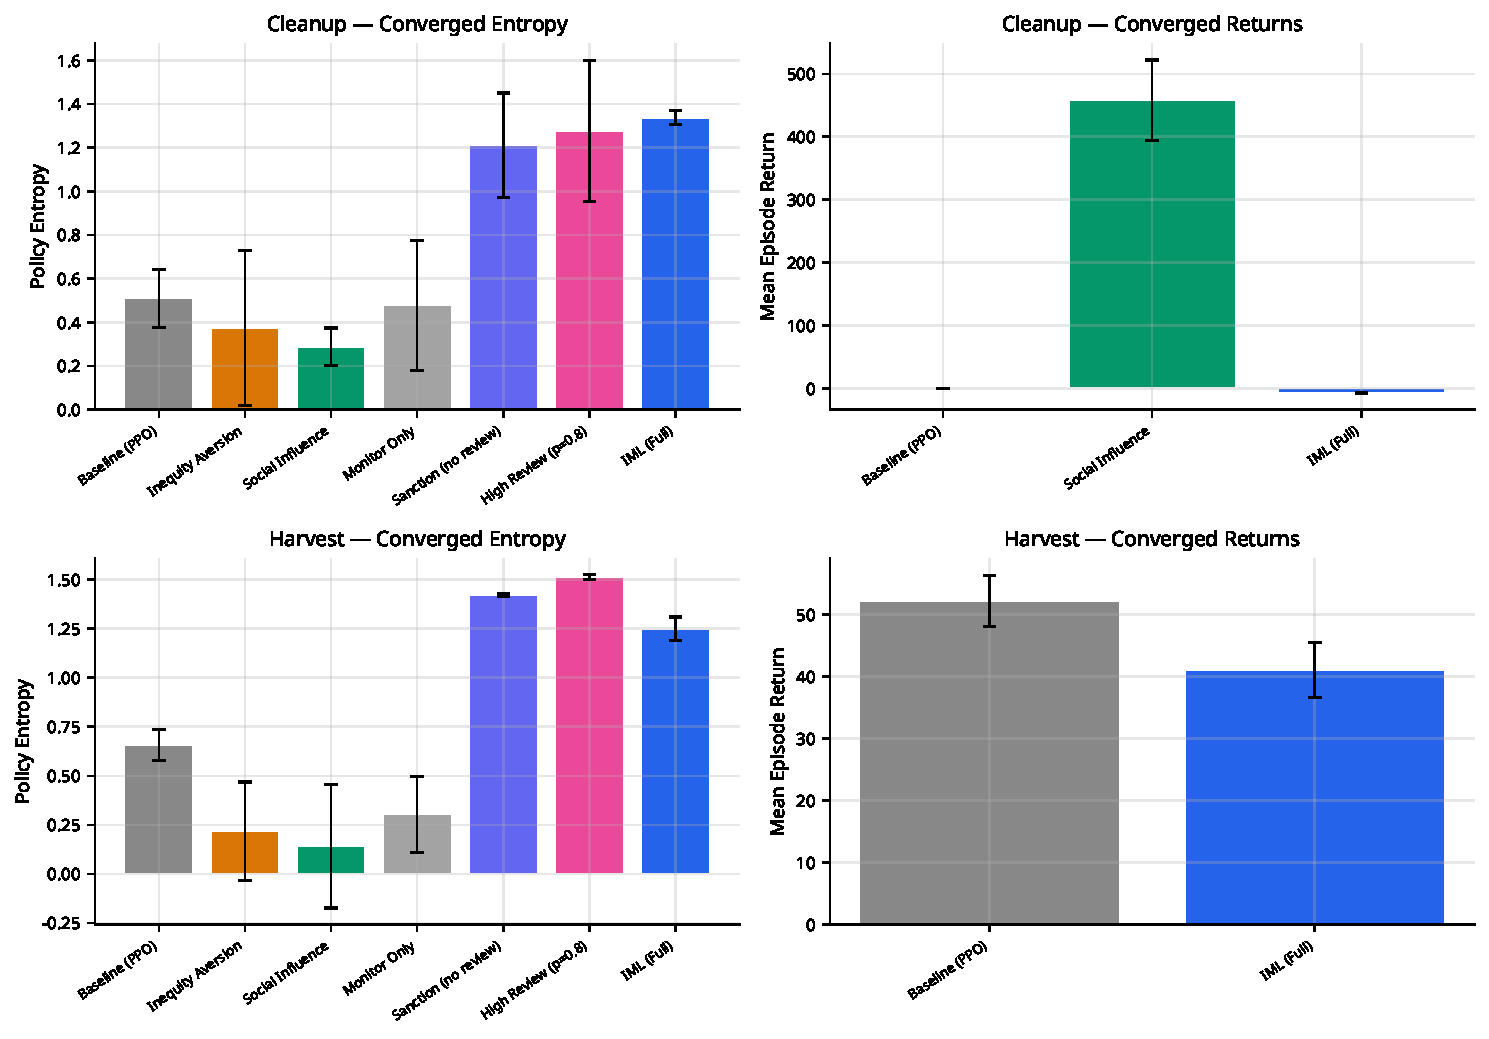
\includegraphics[width=\linewidth]{figures/fig_main_summary.pdf}
\caption{\textbf{Main experimental results.} Top row: \textsc{Cleanup}. Bottom row: \textsc{Harvest}. Left: final policy entropy. Right: mean episode return. IML sustains higher policy entropy than Baseline in both environments, while IA and SI exhibit instability or collapse.}
\label{fig:main_summary}
\end{figure}

In contrast, the external institutional wrapper (IML) maintains more stable optimization dynamics while materially altering policy exploration. As shown in Figure~\ref{fig:entropy_cleanup}, Baseline PPO agents rapidly collapse to deterministic policies (entropy $\approx 0.51$ in \textsc{Cleanup}, $0.66$ in \textsc{Harvest}). IML agents, however, sustain substantially higher entropy throughout training ($1.34$ in \textsc{Cleanup}, $1.25$ in \textsc{Harvest}; Table~\ref{tab:converged_training}). This pattern suggests that the institutional wrapper prevents agents from collapsing into rigid, exploitative strategies and maintains a more exploratory joint policy.

\begin{figure}[!ht]
\centering
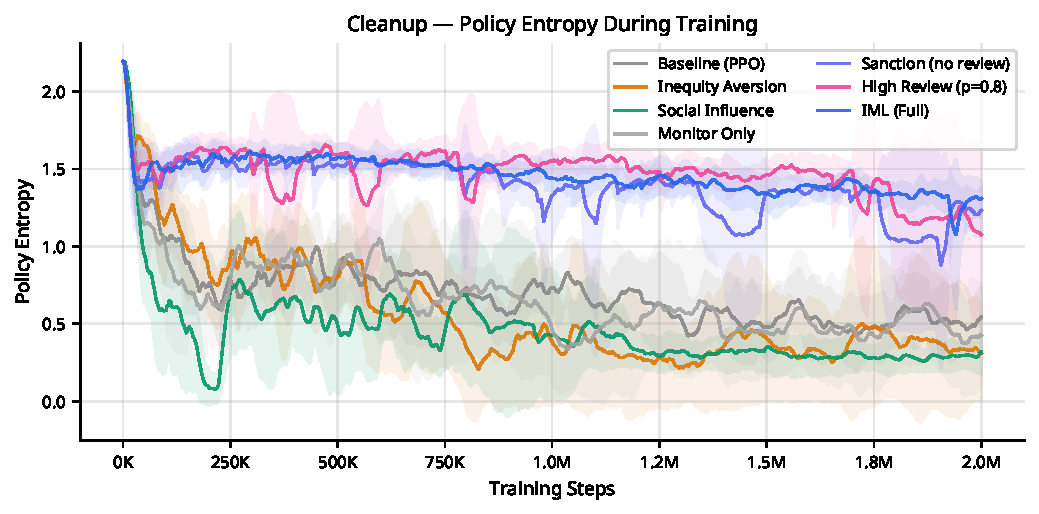
\includegraphics[width=\linewidth]{figures/fig_entropy_cleanup.pdf}
\caption{\textbf{Policy Entropy During Training (\textsc{Cleanup}).} IML and its sanctioning variants maintain high policy entropy (exploration) throughout training, while Baseline, Monitor Only, and SI collapse to deterministic policies.}
\label{fig:entropy_cleanup}
\end{figure}

\begin{table}[htbp]
\caption{Converged training metrics (mean $\pm$ std over 5 seeds, last 20\% of training). Bold indicates best per environment.}
\label{tab:converged_training}
\centering
\footnotesize
\begin{tabular}{llrrr}
\toprule
\textbf{Environment} & \textbf{Condition} & \textbf{Entropy} & \textbf{Value Loss} & \textbf{Clip Frac.} \\
\midrule
  Cleanup & Baseline (PPO) & 0.510 $\pm$ 0.134 & 0.0623 $\pm$ 0.0819 & 0.0829 \\
   & Inequity Aversion & 0.374 $\pm$ 0.357 & 53.71 $\pm$ 80.05 & 0.0484 \\
   & Social Influence & 0.288 $\pm$ 0.086 & 3.12 $\pm$ 0.24 & 0.0362 \\
   & Monitor Only & 0.478 $\pm$ 0.299 & 5.64 $\pm$ 12.48 & 0.0684 \\
   & Sanction (no review) & 1.210 $\pm$ 0.240 & 0.0695 $\pm$ 0.0390 & 0.0987 \\
   & High Review (p=0.8) & 1.276 $\pm$ 0.322 & \textbf{0.0528 $\pm$ 0.0218} & 0.0623 \\
   & IML (Full) & \textbf{1.338 $\pm$ 0.032} & 0.1091 $\pm$ 0.0233 & 0.0967 \\
\midrule
  Harvest & Baseline (PPO) & 0.658 $\pm$ 0.077 & 0.4673 $\pm$ 0.0347 & 0.0615 \\
   & Inequity Aversion & 0.218 $\pm$ 0.251 & 68167.38 $\pm$ 151973.62 & 0.0203 \\
   & Social Influence & 0.140 $\pm$ 0.314 & 16.07 $\pm$ 17.57 & 0.0143 \\
   & Monitor Only & 0.303 $\pm$ 0.192 & 3.50 $\pm$ 7.81 & 0.0390 \\
   & Sanction (no review) & 1.421 $\pm$ 0.007 & 0.0410 $\pm$ 0.0155 & 0.0530 \\
   & High Review (p=0.8) & \textbf{1.514 $\pm$ 0.011} & \textbf{0.0206 $\pm$ 0.0132} & 0.0346 \\
   & IML (Full) & 1.251 $\pm$ 0.059 & 0.4524 $\pm$ 0.0835 & 0.0562 \\
\bottomrule
\end{tabular}
\end{table}


\subsection{Ablation study: isolating institutional mechanisms}

To understand which components of IML drive these effects, we conducted an ablation study (Table~\ref{tab:ablation} and Figure~\ref{fig:ablation_cleanup}). 

\begin{table}[htbp]
\caption{Ablation study: effect of individual IML components on converged training metrics (mean $\pm$ std over 5 seeds).}
\label{tab:ablation}
\centering
\footnotesize
\begin{tabular}{llrr}
\toprule
\textbf{Env.} & \textbf{Condition} & \textbf{Entropy} & \textbf{Value Loss} \\
\midrule
  Cleanup & Baseline (PPO) & 0.510 $\pm$ 0.134 & 0.0623 $\pm$ 0.0819 \\
   & Monitor Only & 0.478 $\pm$ 0.299 & 5.64 $\pm$ 12.48 \\
   & Sanction (no review) & 1.210 $\pm$ 0.240 & 0.0695 $\pm$ 0.0390 \\
   & IML (Full) & 1.338 $\pm$ 0.032 & 0.1091 $\pm$ 0.0233 \\
   & High Review (p=0.8) & 1.276 $\pm$ 0.322 & 0.0528 $\pm$ 0.0218 \\
\midrule
  Harvest & Baseline (PPO) & 0.658 $\pm$ 0.077 & 0.4673 $\pm$ 0.0347 \\
   & Monitor Only & 0.303 $\pm$ 0.192 & 3.50 $\pm$ 7.81 \\
   & Sanction (no review) & 1.421 $\pm$ 0.007 & 0.0410 $\pm$ 0.0155 \\
   & IML (Full) & 1.251 $\pm$ 0.059 & 0.4524 $\pm$ 0.0835 \\
   & High Review (p=0.8) & 1.514 $\pm$ 0.011 & 0.0206 $\pm$ 0.0132 \\
\bottomrule
\end{tabular}
\end{table}


\begin{figure}[!ht]
\centering
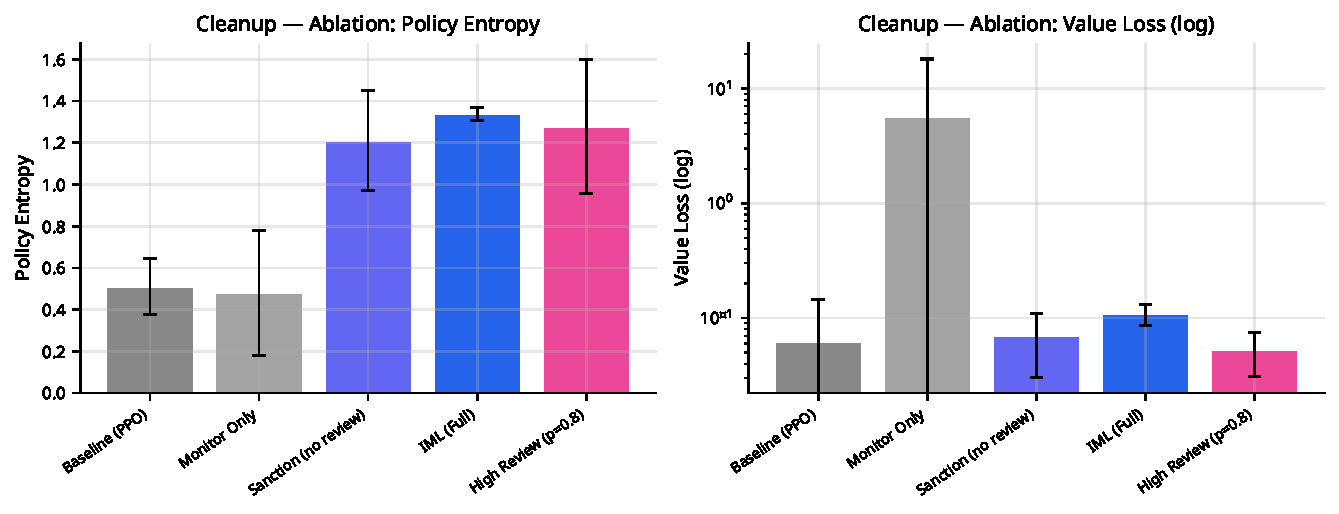
\includegraphics[width=\linewidth]{figures/fig_ablation_cleanup.pdf}
\caption{\textbf{Ablation study (\textsc{Cleanup}).} The Monitor Only condition closely tracks Baseline, indicating that observation alone does not change behavior. The sanction mechanism drives the primary increase in policy entropy, while review adds a smaller modulation.}
\label{fig:ablation_cleanup}
\end{figure}

The results clearly isolate the causal mechanisms of the institution:
\begin{enumerate}
    \item \textbf{Observation is insufficient:} The Monitor Only condition closely tracks the Baseline (entropy $0.48$ vs $0.51$). Simply logging violations without enforcement does not materially alter agent behavior.
    \item \textbf{Sanctions drive exploration:} The Sanction (No Review) condition achieves the vast majority of IML's effect (entropy $1.21$ in \textsc{Cleanup}, $1.42$ in \textsc{Harvest}). The threat of external penalty forces agents to maintain more stochastic policies to avoid predictable violations.
    \item \textbf{Review modulates the effect:} Adding the review mechanism (Full IML) slightly increases entropy in \textsc{Cleanup} ($1.34$) but decreases it in \textsc{Harvest} ($1.25$). Increasing the review probability to $0.8$ (High Review) further modulates this effect. This suggests that the contestability interface is not merely a post-hoc fairness mechanism, but an active institutional parameter that shapes system behavior.
\end{enumerate}

\subsection{Evaluation outcomes and the institutional tax}

While IML improves optimization stability and sustains exploration, it introduces a structural cost under imperfect monitoring. Figure~\ref{fig:episodes_cleanup} shows the episode returns and Gini coefficients for Baseline, SI, and IML.

\begin{figure}[!ht]
\centering
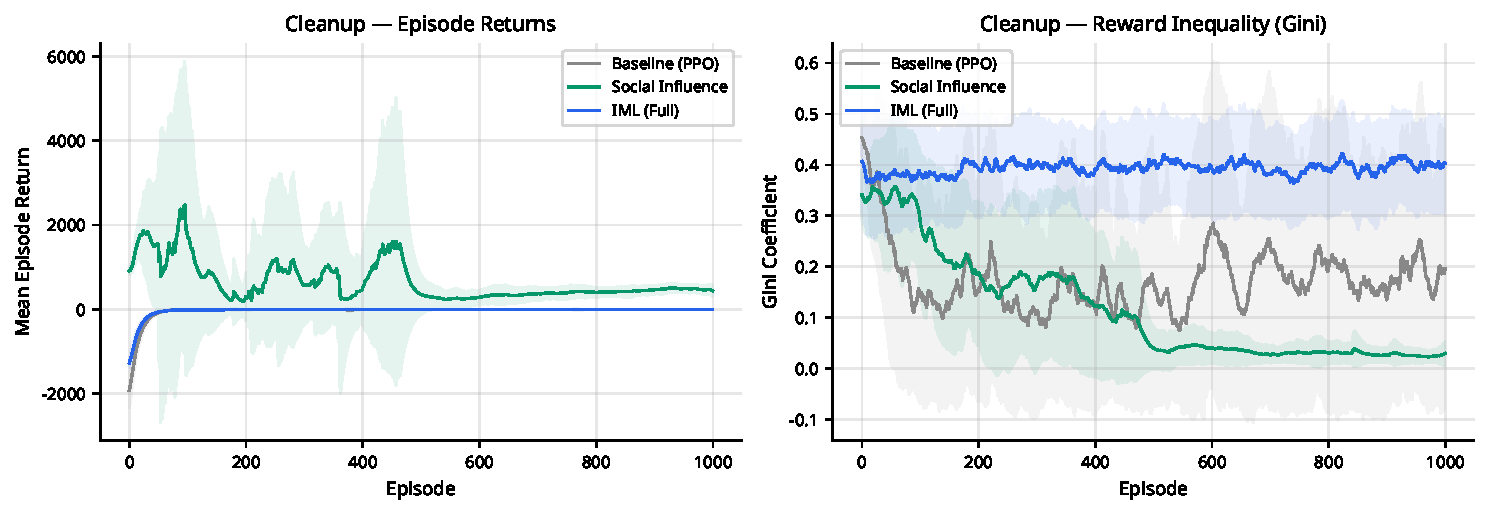
\includegraphics[width=\linewidth]{figures/fig_episodes_cleanup.pdf}
\caption{\textbf{Episode Metrics (\textsc{Cleanup}).} Left: Mean return per agent. Right: Gini coefficient (inequality). IML keeps inequality trajectories more bounded and less volatile than Baseline, but at a higher mean Gini level, and incurs a structural welfare cost due to false-positive sanctions.}
\label{fig:episodes_cleanup}
\end{figure}

In \textsc{Cleanup}, Baseline converges to an approximately zero-return regime. Under IML, mean evaluation return shifts to $-7.63$ per agent (Table~\ref{tab:episode_metrics}). This welfare loss is explained almost entirely by false-positive sanctioning. Because monitoring noise is applied per agent-step, the expected number of false detections per episode scales linearly with the horizon $T$. With $N=5$, $T=2000$, and $p_{\mathrm{fp}}=0.01$, the expected false positives are $\approx 100$ per episode. Even with a $20\%$ review rate overturning erroneous sanctions, the remaining net sanctions impose a persistent ``institutional tax'' on the population.

\begin{table}[htbp]
\caption{Converged episode-level metrics (mean $\pm$ std over 5 seeds, last 200 episodes). Bold indicates best among the reported conditions for each environment.}
\label{tab:episode_metrics}
\centering
\footnotesize
\begin{tabular}{llrr}
\toprule
\textbf{Environment} & \textbf{Condition} & \textbf{Mean Return} & \textbf{Gini Coefficient} \\
\midrule
  Cleanup & Baseline (PPO) & -0.3 $\pm$ 0.5 & 0.1807 $\pm$ 0.0933 \\
   & Social Influence & \textbf{458.4 $\pm$ 63.7} & \textbf{0.0279 $\pm$ 0.0105} \\
   & IML (Full) & -7.6 $\pm$ 0.2 & 0.4001 $\pm$ 0.0054 \\
\midrule
  Harvest & Baseline (PPO) & \textbf{52.2 $\pm$ 4.1} & \textbf{0.1831 $\pm$ 0.0359} \\
   & IML (Full) & 41.1 $\pm$ 4.4 & 0.1922 $\pm$ 0.0190 \\
\bottomrule
\end{tabular}
\end{table}


For \textsc{Harvest}, Table~\ref{tab:episode_metrics} focuses on the direct Baseline--IML welfare comparison; SI's Harvest training behavior is reported in Table~\ref{tab:converged_training}. In \textsc{Cleanup}, the institutional effect on inequality is a volatility effect rather than a mean-improvement effect: IML is tightly concentrated around a higher Gini level, whereas Baseline has lower mean inequality but much larger episode-to-episode variation.

\subsection{Interpretation and interaction design implications}

Taken together, these results support the paper's narrower claim: cooperation mechanisms for human--AI systems should be analyzed not only as reward-design choices, but also as institutions with explicit procedural properties. In these two SSD settings, the internalization baselines were harder to tune robustly, whereas the external IML wrapper remained stable but introduced measurable procedural costs.

From an interaction design perspective (Section~\ref{sec:interaction_design}), the ablation study underscores the critical importance of the contestability interface. In our simulated experiments, the review process is automated and probabilistic. In real-world deployments, however, the review would involve human stakeholders interacting with the ledger through a multimodal interface---examining evidence, formulating appeals, and receiving outcomes. 

The quality of this interaction directly affects the effective review rate ($p_{\mathrm{review}}$) and, consequently, the magnitude of the institutional tax. Poorly designed review interfaces that are cognitively burdensome would lower the effective review rate (closer to the Sanction-No-Review ablation) and increase false-positive harm. By contrast, clearer interfaces and more efficient appeal processes (closer to the High Review ablation) would mitigate these costs while preserving the behavioral benefits of the institution.

A capacity-constrained review pipeline would generally worsen this picture. If appeal volume exceeds reviewer throughput, the effective review process is not only lower $p_{\mathrm{review}}$ but also larger settlement delay $D$, and Section~\ref{sec:delay} implies that both changes push the system toward higher residual sanction burden. The present simulations vary $p_{\mathrm{review}}$ while keeping $D$ fixed, so they should be interpreted as a lower-dimensional proxy for review bandwidth rather than as a full model of queueing or institutional gridlock. Appendix~\ref{app:sensitivity} complements this interpretation with an evaluation-only sweep over $p_{\mathrm{fp}}$ and $p_{\mathrm{review}}$, showing that lower false-positive rates and higher review probabilities reduce sanction overhead and partially restore welfare when the learned policy is held fixed.

Given $n=5$ training seeds per condition, the inferential results in Table~\ref{tab:statistical_tests} should be read as exploratory. We therefore rely primarily on directional consistency across seeds, uncertainty intervals, effect sizes, and ablation structure rather than on binary significance claims.

\begin{table}[htbp]
\caption{Statistical comparison of IML against baselines (converged entropy). Mann-Whitney $U$ test with Holm-Bonferroni correction. $d$: Cohen's $d$; $\delta$: Cliff's delta.}
\label{tab:statistical_tests}
\centering
\footnotesize
\begin{tabular}{llrrrrl}
\toprule
\textbf{Env.} & \textbf{Comparison} & \textbf{$U$} & \textbf{$p$} & \textbf{$p_{\mathrm{adj}}$} & \textbf{$d$} & \textbf{Sig.} \\
\midrule
  Cleanup & IML vs Baseline (PPO) & 25 & 0.0079 & 0.0952 & 8.49 & n.s. \\
  Cleanup & IML vs Inequity Aversion & 25 & 0.0079 & 0.0952 & 3.80 & n.s. \\
  Cleanup & IML vs Social Influence & 25 & 0.0079 & 0.0952 & 16.15 & n.s. \\
  Cleanup & IML vs Monitor Only & 25 & 0.0079 & 0.0952 & 4.04 & n.s. \\
  Cleanup & IML vs Sanction (no review) & 17 & 0.4206 & 0.8413 & 0.74 & n.s. \\
  Cleanup & IML vs High Review (p=0.8) & 11 & 0.8413 & 0.8413 & 0.27 & n.s. \\
  Harvest & IML vs Baseline (PPO) & 25 & 0.0079 & 0.0952 & 8.62 & n.s. \\
  Harvest & IML vs Inequity Aversion & 25 & 0.0119 & 0.0952 & 5.66 & n.s. \\
  Harvest & IML vs Social Influence & 25 & 0.0079 & 0.0952 & 4.91 & n.s. \\
  Harvest & IML vs Monitor Only & 25 & 0.0079 & 0.0952 & 6.67 & n.s. \\
  Harvest & IML vs Sanction (no review) & 0 & 0.0079 & 0.0952 & -4.05 & n.s. \\
  Harvest & IML vs High Review (p=0.8) & 0 & 0.0079 & 0.0952 & -6.18 & n.s. \\
\bottomrule
\end{tabular}
\end{table}


\subsection{Per-agent fairness and false-positive burden}
\label{sec:fairness}

A central concern for accountability institutions is how enforcement burdens are distributed across agents. Aggregate welfare can mask whether some agents bear disproportionate false-positive costs, even when mean outcomes appear acceptable. To address this, we analyze IML ledger records at the agent level, tracking flagged sanction events, true violations, false positives, and overturned cases across runs.

Table~\ref{tab:fairness} reports the per-agent enforcement profile in both environments. Here, \emph{Sanctions/ep.} denotes pre-review flagged sanction events per agent per episode; \emph{TP/ep.} and \emph{FP/ep.} partition those flagged events into true violations and false positives, and \emph{Overturn Rate} is the fraction of flagged events later reversed in review. In these symmetric benchmark settings, the pre-review burden is nearly uniform across agents. The sanction Gini coefficient is $0.0040 \pm 0.0005$ in \textsc{Cleanup} and $0.0033 \pm 0.0013$ in \textsc{Harvest}, and the per-agent flagged counts cluster tightly around $20.6$ events per episode.

\input{tables/tab_fairness.tex}

Figure~\ref{fig:fairness_per_agent_boxplot} visualizes the per-agent sanction distribution. The narrow spread across agents is consistent with the structural symmetry of the monitored rule and monitoring process in these environments. This result is useful, but it should be interpreted narrowly: it does not imply that institutional fairness is guaranteed under heterogeneous roles, asymmetric observability, or differential monitoring in real deployments.

\begin{figure}[!ht]
\centering
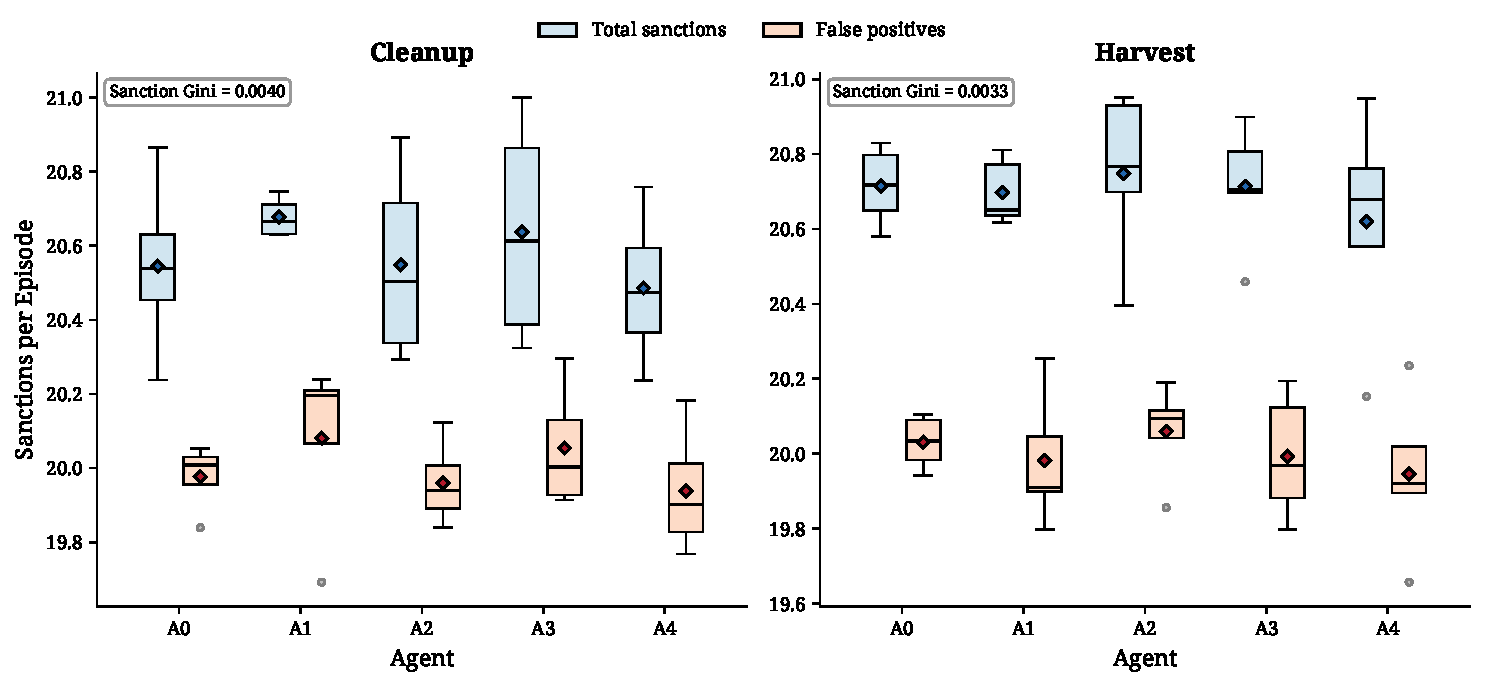
\includegraphics[width=\linewidth]{figures/fairness_per_agent_boxplot.pdf}
\caption{\textbf{Per-agent sanction distribution.} Left: \textsc{Cleanup}. Right: \textsc{Harvest}. In these symmetric environments, flagged sanction counts and false-positive burden remain tightly clustered across the five agents.}
\label{fig:fairness_per_agent_boxplot}
\end{figure}

The ledger also reveals an important temporal shift. Figure~\ref{fig:fairness_temporal_dynamics} shows that true-positive sanctions are concentrated early in training, when agents still violate the monitored rule. As policies adapt, true violations fall sharply, but sanctions do not disappear because residual enforcement is increasingly driven by monitoring error.

\begin{figure}[!ht]
\centering
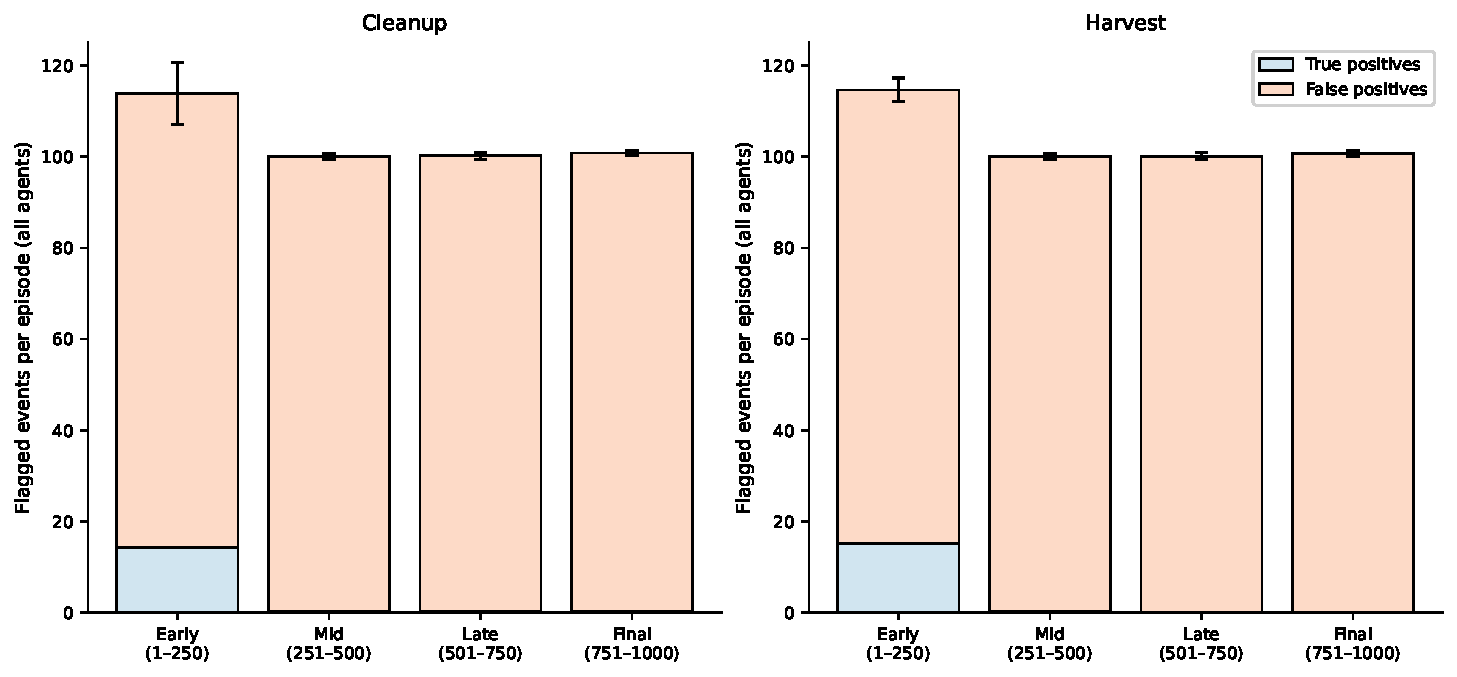
\includegraphics[width=\linewidth]{figures/fairness_temporal_dynamics.pdf}
\caption{\textbf{Temporal composition of sanctions.} Early in training, true violations contribute materially to sanctions. Later, as compliance improves, the remaining burden is dominated by false positives.}
\label{fig:fairness_temporal_dynamics}
\end{figure}

Figure~\ref{fig:fairness_fp_rate_evolution} makes this transition explicit. As agents learn to comply, the fraction of sanctions that are false positives rises toward 100\%. This is the same long-horizon ``institutional tax'' predicted by the incentive analysis: once real violations become rare, even a small per-step false-positive rate can dominate the remaining enforcement burden.

\begin{figure}[!ht]
\centering
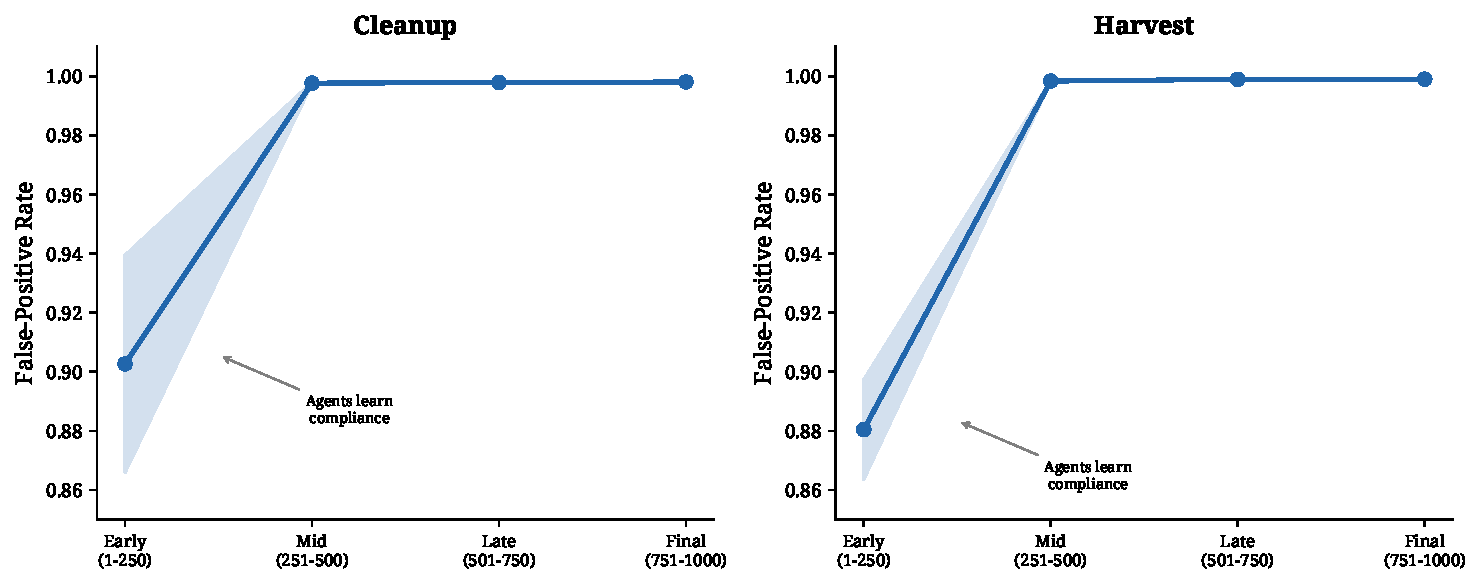
\includegraphics[width=\linewidth]{figures/fairness_fp_rate_evolution.pdf}
\caption{\textbf{False-positive rate over training.} As true violations become rarer, the fraction of sanctions attributable to false positives approaches 100\%, reinforcing the need for calibrated review and error budgeting.}
\label{fig:fairness_fp_rate_evolution}
\end{figure}

Together, these results refine the paper's fairness claim. In the present symmetric benchmarks, IML does not concentrate sanction burden on particular agents. The more durable lesson, however, is temporal rather than distributive: mature compliance regimes make review and appeal more important, not less, because the residual burden increasingly reflects measurement error rather than genuine violations.


\section{Case vignettes: what IML looks like in human--AI integration}
\label{sec:cases}

To make the institutional questions concrete, we outline four vignettes that illustrate how IML could be instantiated in human--AI integration. These are not empirical case studies. Rather, they are structured scenarios meant to clarify where design choices concentrate ethical risk, what kinds of evidence and recourse are feasible, and how the same technical primitives can support either accountable governance or coercive control depending on how they are scoped and governed.

\subsection{Platform community governance: moderation and harassment}

Consider a large platform that uses AI assistants to support harassment mitigation, misinformation moderation, and community rule enforcement. The socio-technical system is inherently multi-agent: users, creators, recommendation/ranking components, automated classifiers, reporting tools, and human moderators interact repeatedly, often under asymmetric information. Norms are expressed through community standards (e.g., harassment, coordinated abuse, doxxing), but these standards are contested, context-dependent, and frequently require interpretation rather than mechanical application.

In this setting, an IML-style institution is attractive because it can make enforcement \emph{inspectable} rather than merely effective. The design challenge is to define monitoring scope without collapsing into pervasive surveillance. Monitoring must specify what signals are collected (content, metadata, interaction graphs) and justify these flows under contextual integrity constraints \citep{Nissenbaum2004}. Evidence pipelines must avoid opacity failures in which users cannot understand what evidence was used or why a classification was treated as actionable \citep{Burrell2016Opacity}. Contestability must be treated as a core mechanism property rather than a customer-support add-on: users need a practicable path to appeal takedowns or sanctions, and explanations must be intelligible and matched to the kinds of mistakes the system makes \citep{Lee2019ProceduralJustice}. Finally, the institution must explicitly consider power and chilling effects. Even when enforcement improves aggregate safety, monitoring that is experienced as pervasive or unpredictable can deter participation and reshape expressive behavior \citep{Lyon2007Surveillance,Foucault1977DisciplinePunish}.

A concrete instantiation can be deliberately minimalist. Instead of ``collect everything'' logging, the ledger can record (i) the specific norm invoked (policy clause and version), (ii) a pointer to the content/action at issue, (iii) the evidence features actually relied upon (e.g., classifier scores, report provenance, limited contextual signals), and (iv) the settlement outcome (warning, takedown, time-limited restriction) with graduated escalation \citep{Ostrom1990}. Where content retention is high-risk, the ledger can store commitments/hashes and access-controlled references rather than full payloads. Crucially, the contestation interface should expose the invoked norm and provide a path to human review, because legitimacy depends on being heard and having recourse, not only on outcome accuracy \citep{Tyler1990,Lee2019ProceduralJustice}. The same infrastructure can become illegitimate if monitoring scope expands without explicit boundary-setting and oversight; in this vignette, the main value of IML is precisely that it makes boundaries and procedures governable.

\subsection{Enterprise agentic workflows: policy compliance and data access}

Organizations increasingly deploy agentic assistants that plan tasks, call tools, query internal databases, and coordinate work across teams. Here, ``cooperation'' often means compliance with access controls, adherence to data-minimization policies, truthful reporting of uncertainty, and non-circumvention of safety constraints. The relevant multi-agent ecology includes employees, teams, contractors, internal systems, AI components, and security/compliance functions.

IML naturally fits this environment as an accountability layer for norm-relevant events such as access requests, data exports, and tool calls, with settlement delayed to support review. The ethical risk, however, is acute: workplace logging can drift into surveillance, and auditability can be repurposed for performance discipline rather than policy compliance \citep{Zuboff2019,Lyon2007Surveillance}. Accordingly, governance must specify who can access logs, what is retained, and how individuals can contest interpretations of logged events, especially where false positives can trigger reputational or employment harm.

A defensible instantiation treats IML as a \emph{policy compliance institution} rather than a productivity-monitoring apparatus. This implies role-based access to logs, strict retention limits, and aggregation where feasible (e.g., counts of policy-relevant events rather than raw content), along with a clear separation between security monitoring and HR/performance evaluation. Contestability should be operational: employees should be able to challenge whether a logged event was truly a violation (including disputing false positives) and whether the applied settlement was proportionate, with documented resolution timelines. In such settings, the ledger’s primary governance value is to enable audit and incident reconstruction without normalizing pervasive workplace surveillance.

\subsection{Autonomous fleets: shared safety norms}

Robot fleets in warehouses, delivery, or medical logistics share resources and coordinate under safety and efficiency constraints. Cooperation in this vignette takes the form of safe spacing, deconfliction, right-of-way adherence, and compliance with priority rules, with repeated interactions and potentially high-stakes externalities.

Here, an IML-style institution can act as a shared ``incident ledger'' that supports both deterrence and post hoc investigation. The ledger can record norm-relevant events (near-misses, rule violations, overrides), while settlement can implement graded responses such as capability throttling, mandatory safety re-calibration, or temporary access restrictions after repeated unsafe behavior. This is aligned with proposals for accountable recording in autonomous systems (ethical ``black boxes'') \citep{WinfieldJirotka2017}. Because these deployments are safety-critical and organizationally embedded, meaningful human control requires that humans can override institutional actions and audit why they occurred, and that responsibility attribution is supported by usable records \citep{Santoni2018MHC,Shneiderman2020HCAI}.

A concrete instantiation should prioritize investigability without maximizing surveillance. The ledger can store time-bounded sensor snapshots (subject to privacy limits), policy and firmware versions, and a trace of actions leading to near-misses, enabling reproducible incident reconstruction. Settlement is often better framed as capability and safety management (e.g., throttling after repeated violations) rather than purely punitive transfers, reducing incentives to hide incidents and aligning with safety governance norms. As in other vignettes, monitor error rates and settlement rules should be audited periodically: wrongful ``incidents'' can trigger costly downtime and erode trust in both the robots and the institution.

\subsection{Public-sector services: eligibility, compliance, and the risk of ``automated punishment''}

Public-sector agencies increasingly rely on data-driven systems to allocate scarce resources, flag fraud, and prioritize service provision. The socio-technical system is multi-agent: citizens, caseworkers, contractors, and decision-support models interact over time. These settings are institutionally hard because power asymmetries are large, stakes are high, and procedural legitimacy is not optional. Empirical accounts caution that automated systems can produce punitive error cascades when monitoring and enforcement are opaque, unaccountable, or disconnected from meaningful recourse \citep{Eubanks2018AutomatingInequality,ONeil2016WMD}.

If IML were deployed at all in this domain, it should be used to \emph{raise} the procedural floor rather than accelerate sanctions. Evidence standards must be explicit (what counts as actionable evidence, how uncertainty is represented, and what human review is required), and due process must be designed for real access, including offline appeal pathways for people with limited digital connectivity or literacy. Monitoring scope must be justified against contextual expectations and the risk of surveillance harms \citep{Lyon2007Surveillance}. A ledger can help conditionally by forcing documentation and contestability: each flag is tied to a norm, an evidence trail, a settlement rule, and a review outcome, and the institution can be audited for error rates and disparate burdens. Yet the same infrastructure can be used to intensify monitoring or routinize punitive automation; this vignette therefore underscores a boundary condition for IML: in high power-asymmetry settings, the legitimacy constraints in Section~\ref{sec:falsepos} and the governance lifecycle in Section~\ref{sec:governance} are baseline requirements rather than optional best practices.


\section{Governance integration: from principles to practice}
\label{sec:governance}

High-level ethics principles are widespread yet repeatedly fail to constrain practice when they are not institutionalized into roles, procedures, and inspectable artifacts \citep{Jobin2019EthicsGuidelines,Mittelstadt2019Principles}. IML is designed to support such institutionalization by making enforcement \emph{procedural} and \emph{auditable}: norms are explicit, monitoring scope is governable, settlements are logged, and review outcomes are recorded. This section describes how an IML deployment can be integrated into governance processes in a way that is operational rather than aspirational.

\subsection{Lifecycle governance}

Institutional mechanisms require lifecycle governance because norms, evidence pipelines, and organizational practices evolve. We therefore propose a governance lifecycle with five linked phases (Figure~\ref{fig:lifecycle}). The lifecycle begins with \emph{participatory norm-setting}, in which the norm predicate $v$ and settlement goals are defined with relevant stakeholders rather than silently encoded. It continues with a \emph{pre-deployment impact assessment} that documents anticipated harms, monitoring scope, contestability pathways, and mitigation plans in the style of algorithmic impact assessment practice \citep{Metcalf2021AIA,Selbst2021AIA}. Deployment should then occur \emph{with audit hooks by design}: evidence and settlements are logged, error metrics are measured and tracked, and access/retention rules are enforced as governance constraints rather than engineering defaults. Once deployed, IML must support \emph{ongoing redress} through functioning appeals and dispute resolution, including aggregate reporting on outcomes and error burdens. Finally, the institution must be \emph{audited and updated} through internal and/or external review, including analysis of appeals and revision of norms and settlement policies when evidence or stakeholder feedback indicates drift, abuse potential, or unjust burdens \citep{Raji2020Auditing,Sandvig2014AuditingAlgorithms}. The key governance claim is that institutions should be revisable: contestability is not merely about individual cases, but about the ability to change institutional rules when they fail.

\begin{figure}[t]
\centering
\begin{tikzpicture}[font=\small, node distance=1.3cm]
\tikzstyle{b}=[draw, rounded corners, align=center, inner sep=6pt]
\node[b] (n) {Participatory\\ norm-setting};
\node[b, below=.6cm of n] (a) {Impact\\ assessment};
\node[b, right=.6cm of a] (d) {Deployment\\ \& monitoring};
\node[b, right=.6cm of d] (r) {Redress\\ \& appeals};
\node[b, above=.6cm of r] (u) {Audit\\ \& update};

\draw[-{Latex[length=3mm]}] (n) -- (a);
\draw[-{Latex[length=3mm]}] (a) -- (d);
\draw[-{Latex[length=3mm]}] (d) -- (r);
\draw[-{Latex[length=3mm]}] (r) -- (u);
\draw[-{Latex[length=3mm]}] (u.west) to[bend right=15] (n.east);
\end{tikzpicture}
\caption{Governance lifecycle for IML: participatory norm-setting, impact assessment, deployment and monitoring, redress, and audit/update. The loop emphasizes that institutions should be revisable in response to evidence and stakeholder feedback.}
\label{fig:lifecycle}
\end{figure}

\subsection{Alignment with standards and regulation}

IML can support compliance-oriented risk management by producing inspectable artifacts that many frameworks increasingly expect: explicit monitoring policies, settlement rules, auditable logs, and documented error rates \citep{NIST2023AIRMF,ISO23894,OECDAI2019,EU2024AIAct}. In practice, these artifacts can help organizations meet requirements for transparency, accountability, and post-incident reconstruction. However, alignment should not be treated as a check-box exercise: an institution can satisfy formal documentation requirements while still being illegitimate for affected communities. Accordingly, standards alignment should be treated as necessary but not sufficient; legitimacy depends on whether affected parties experience contestability, proportionality, and contextual integrity in practice.

\subsection{From framework requirements to concrete artifacts}

To avoid ``principles without practice'' \citep{Mittelstadt2019Principles}, IML deployments should produce artifacts that can be inspected by reviewers, auditors, and affected communities. Table~\ref{tab:rmfmap} illustrates one natural mapping from IML outputs to common risk-management functions, using the NIST AI RMF categories as a convenient organizing frame \citep{NIST2023AIRMF}. The intent is not superficial compliance, but operational hooks that allow institutions to be scrutinized, challenged, and revised when they fail.

\begin{table}[t]
\centering
\small
\begin{tabular}{p{0.22\linewidth} p{0.72\linewidth}}
\toprule
\textbf{Governance function} & \textbf{IML artifacts that support it} \\
\midrule
\textbf{Govern} & Norm specification $v$ with provenance; settlement rule $\Sigma$ with proportionality bounds; documented oversight roles; appeal policy; retention and access controls. \\
\textbf{Map} & Context-of-use statement; stakeholder analysis; monitoring scope aligned with contextual integrity \citep{Nissenbaum2004}; threat model and failure modes (Section~\ref{sec:failure}). \\
\textbf{Measure} & Monitor error rates $(p,q)$; appeal accuracy $\alpha$; wrongful penalty estimates; privacy leakage measures; welfare and legitimacy metrics (Table~\ref{tab:metrics}). \\
\textbf{Manage} & Update and rollback procedures for $M$ and $\Sigma$; audit schedule; incident response plan; versioned logs enabling post-hoc analysis and redress \citep{Raji2020Auditing}. \\
\bottomrule
\end{tabular}
\caption{Illustrative mapping from IML artifacts to governance functions. The goal is not superficial compliance but operational hooks that make institutions inspectable and revisable.}
\label{tab:rmfmap}
\end{table}

A practical implication is that IML should ship with a \emph{minimum viable governance package}---a baseline set of commitments that make the institution auditable and contestable even under constrained organizational capacity. At minimum, this package should document the enforced norms and their justification (including stakeholder participation and dissent handling); the monitoring scope, data sources, retention limits, and access controls; the settlement logic, sanction bounds, and the points where humans are in the loop; measured error rates and a plan for continuous monitoring of those errors; a functioning appeal and redress mechanism accompanied by aggregate statistics on reversals and resolution times; and an update process that prevents silent changes to institutional rules and enables rollback when harm is detected. These artifacts are not merely administrative: they are the concrete mechanisms by which institutions become governable rather than opaque.

By requiring explicit artifacts and revision pathways, IML also directly targets failure patterns documented in critiques of opaque algorithmic governance, where automated decisions are difficult to contest, error burdens cascade, and institutional accountability is diffuse \citep{ONeil2016WMD,Eubanks2018AutomatingInequality}.


\section{Limitations and open problems}
\label{sec:limits}

Several limitations of the current work should be acknowledged.

\begin{itemize}
    \item While we articulate interaction design principles for contestable AI institutions (Section~\ref{sec:interaction_design}), we do not evaluate these principles with human participants. A user study examining how stakeholders interact with the auditable ledger, how effectively they can contest false positives, and how the interface design affects perceived procedural justice would materially strengthen the empirical grounding of our interaction design claims. This is a priority for future work.

    \item Our empirical evaluation now includes direct quantitative comparisons against inequity aversion and social influence, which helps position IML relative to representative internalization approaches. The baseline set remains selective, however, and does not yet include contract-based approaches, additional norm-aware methods, or environment-specific non-learning baselines.

    \item The evaluation uses two environments with a single narrow rule. This choice was intentional because it isolates monitoring error and due-process effects, but it leaves open how IML behaves under more contested norms, multiple simultaneous rules, and richer interaction dynamics.

    \item The review and appeal channel is simulated probabilistically rather than implemented as an actual human-in-the-loop interaction. The effective review rate in real deployments would depend on the quality of the contestability interface, the cognitive load on reviewers, and the volume of appeals. Capacity bottlenecks could also create queues and longer settlement delays, which our simulations do not model directly.

    \item The simulations should be read as a focused pilot study. Five training seeds per condition are sufficient to surface large directional effects and failure modes, but they are still limited for strong claims about stability, tail behavior, or corrected statistical significance. Future work should expand the seed count, broaden substrates, and report pre-specified reliability metrics such as collapse frequency, variance reduction, and outlier sensitivity.

    \item We now report per-agent sanction and false-positive burden, and in these symmetric environments the burden is nearly uniform across agents. That result should not be overgeneralized: future work should test whether sanctions, reversals, or review delays concentrate on particular agents, roles, states, or demographic groups when monitoring is heterogeneous or strategically manipulated.
\end{itemize}

This paper is deliberately scoped as a framework contribution with pilot experiments: it argues for institutional cooperation mechanisms as a governance-relevant alternative to covert influence, formalizes a minimal IML wrapper, and demonstrates empirically how monitoring error can dominate welfare in long-horizon settings. Several limitations and open problems follow directly from this scope.

First, our incentive analysis is intentionally conservative. The one-shot deviation deterrence bound is designed as an auditable check rather than a full characterization of strategic behavior. Equilibrium analysis in partially observable Markov games with heterogeneous learning dynamics, delayed settlement, and endogenous monitoring remains technically challenging, and our bounds do not capture the richness of multi-step deviations, coordinated deviations, or equilibrium selection effects.

Second, norm specification is not a purely technical problem. Norms are value-laden and contested; even when an institution is transparent, disagreement can persist about what should count as a violation, what evidence is sufficient, and what sanctions are legitimate. Participatory and value-sensitive approaches are therefore necessary, but operationalizing such participation at scale---especially across heterogeneous communities and cultures---remains difficult and politically fraught \citep{FriedmanKahnBorning2002}.

Third, institutional design does not eliminate power. Transparent institutions can still be captured by powerful actors, and procedural features can be implemented in ways that are formally present but substantively ineffective. Meaningful checks and balances, credible oversight, and enforceable constraints on operators are therefore essential for any real deployment, yet such governance capacity varies widely across organizations and jurisdictions.

Fourth, monitoring changes behavior beyond deterrence. Monitoring can produce chilling effects that reduce exploration, creativity, and willingness to engage, which is especially salient for human--AI collaboration and expressive domains \citep{Lyon2007Surveillance}. Even when monitoring improves aggregate welfare, these dignitary and autonomy costs can undermine legitimacy, and they are not easily captured by standard MARL benchmarks.

Finally, legitimacy measurement itself is a moving target. Survey-based legitimacy metrics can be gamed, influenced by framing, or divorced from longer-term institutional experience. For this reason, legitimacy evaluation likely requires mixed methods, longitudinal observation, and attention to how institutions interact with organizational incentives and social power rather than relying on short-run proxies.

\subsection{Research agenda: interaction design for accountable AI institutions}

The interaction design challenges identified in this paper suggest several concrete research directions:
\begin{enumerate}[leftmargin=*]
\item \textbf{Multimodal evidence presentation.} How should complex multi-agent trajectories be visualized to support human review of institutional decisions? What combination of textual logs, spatial visualizations, and temporal replays is most effective for different stakeholder roles?
\item \textbf{Contestability interface evaluation.} What interface designs minimize the cognitive burden of contesting false positives while maintaining the integrity of the appeal process? How does the friction of the appeal interface affect the effective review rate and, consequently, system-level welfare?
\item \textbf{Adaptive monitoring interfaces.} Can the monitoring interface be designed to adapt its sensitivity and reporting based on the observed false-positive rate and the capacity of the review system, creating a feedback loop between interaction design and institutional performance?
\item \textbf{Cross-cultural interaction norms.} How do cultural differences in attitudes toward authority, contestation, and procedural justice affect the design requirements for accountability interfaces in global AI deployments?
\end{enumerate}

\subsection{Research agenda: institutions for agentic ecosystems}

Despite these limitations, IML suggests a concrete interdisciplinary research program for agentic ecosystems in which humans and AI components interact repeatedly under partial observability and power asymmetries. A first priority concerns legitimacy under partial automation: which combinations of explanation, appeal, and outcome control produce stable perceptions of legitimacy when enforcement is partly automated, and how do these procedural features interact with outcome quality over time \citep{Tyler1990,Lee2019ProceduralJustice}? A second priority concerns institutional pluralism and conflict. Digital systems increasingly operate under overlapping communities, jurisdictions, and rule systems; understanding how institutions behave when norms conflict---and how ``nested enterprises'' should be implemented in digital form---is central for practical deployment \citep{Ostrom1990}.

A third priority is privacy-preserving monitoring. Institutional enforcement requires evidence, yet the evidence required for accountability must be balanced against contextual integrity and the risk of surveillance harms \citep{Nissenbaum2004,Lyon2007Surveillance}. This motivates research on what minimal evidence suffices for legitimate enforcement, how to protect evidence while enabling audit, and how to design monitoring scopes that are technically enforceable rather than aspirational. A fourth priority concerns learning dynamics and Goodhart effects: learning agents will adapt to institutional incentives over long horizons, so institutions must detect and correct gaming, proxy exploitation, and feedback-loop pathologies, ideally with auditable diagnostics rather than opaque patching.

Finally, power and capture must be treated as design constraints, not externalities. Future work should examine what checks and balances reduce institutional capture by powerful actors, what transparency is necessary for meaningful external oversight, and how auditing and redress can be made credible when incentives to conceal error are strong \citep{Raji2020Auditing}. Addressing these questions is essential for connecting optimization-centric accounts of cooperation with institution-centered governance in socio-technical systems.

As a closing perspective, across the conceptual framing, incentive checks, and SSD evidence, a consistent empirical lesson emerges: \emph{measurement error is first-order} for institutional cooperation mechanisms. When monitoring is applied at the granularity of agent-steps and decisions are delayed, even small false-positive rates can accumulate into predictable welfare losses and unequal burdens unless they are explicitly budgeted, procedurally mitigated, and audited. For this reason, IML should be read less as a finished governance solution and more as a research framework with pilot empirical evidence: a way to make cooperation interventions legible as institutions with tunable error budgets, contestability pathways, and accountability artifacts, enabling systematic study of the welfare--legitimacy trade-offs that determine whether human--AI cooperation mechanisms are acceptable in practice.

\section{Conclusion}

As AI systems become more deeply integrated into socio-technical settings, the design of accountability mechanisms becomes as important as the underlying learning algorithms. In this paper, we conceptualize and formalize the Institutional Monitoring and Ledger (IML) framework as an institutional wrapper for cooperative multi-agent settings. By adding explicit monitoring, logging, review, and contestability around the base Markov game, IML turns cooperation control into an inspectable institutional process rather than a hidden modification of agent objectives.

Our analysis and pilot experiments in sequential social dilemmas support three main conclusions. First, in these settings, an external institutional layer can alter learning dynamics in ways that representative internalization baselines did not reproduce robustly. Second, measurement error and due-process design become first-order determinants of welfare and legitimacy: over long horizons, false positives generate an institutional tax unless review, sanction magnitude, and delay are carefully calibrated. Third, the added agent-level analysis shows that sanction burden is nearly uniform in these symmetric benchmark environments, while the temporal composition of sanctions shifts toward residual false positives as compliance improves.

The paper therefore argues for treating cooperation mechanisms as institution-design problems, not only reward-design problems. Future work should broaden the empirical substrate, add human-subject evaluation, model capacity-constrained review more directly, and test fairness under heterogeneous monitoring and more contested norms.

\vspace{6pt} 

%%%%%%%%%%%%%%%%%%%%%%%%%%%%%%%%%%%%%%%%%%
%% optional
%\supplementary{The following supporting information can be downloaded at:  \linksupplementary{s1}, Figure S1: title; Table S1: title; Video S1: title.}

% Only for journal Methods and Protocols:
% If you wish to submit a video article, please do so with any other supplementary material.
% \supplementary{The following supporting information can be downloaded at: \linksupplementary{s1}, Figure S1: title; Table S1: title; Video S1: title. A supporting video article is available at doi: link.}

% Only used for preprtints:
% \supplementary{The following supporting information can be downloaded at the website of this paper posted on \href{https://www.preprints.org/}{Preprints.org}.}

% Only for journal Hardware:
% If you wish to submit a video article, please do so with any other supplementary material.
% \supplementary{The following supporting information can be downloaded at: \linksupplementary{s1}, Figure S1: title; Table S1: title; Video S1: title.\vspace{6pt}\\
%\begin{tabularx}{\textwidth}{lll}
%\toprule
%\textbf{Name} & \textbf{Type} & \textbf{Description} \\
%\midrule
%S1 & Python script (.py) & Script of python source code used in XX \\
%S2 & Text (.txt) & Script of modelling code used to make Figure X \\
%S3 & Text (.txt) & Raw data from experiment X \\
%S4 & Video (.mp4) & Video demonstrating the hardware in use \\
%... & ... & ... \\
%\bottomrule
%\end{tabularx}
%}

%%%%%%%%%%%%%%%%%%%%%%%%%%%%%%%%%%%%%%%%%%
\authorcontributions{Conceptualization, S.A.; methodology, S.A.; software, S.A.; validation, S.A.; formal analysis, S.A.; investigation, S.A.; data curation, S.A.; writing: original draft preparation, S.A.; writing: review and editing, S.A.; visualization, S.A. The author has read and agreed to the published version of the manuscript.}

\funding{This research received no external funding.}% The APC was funded by the author.}

\institutionalreview{Not applicable.}

\informedconsent{Not applicable.}

\dataavailability{The code, configuration files, and scripts supporting the findings of this study are available at \url{https://github.com/alqithami/IML}. The results reported in the manuscript can be reproduced by running the provided pipeline; all data are generated via simulation.}

\acknowledgments{The author thanks the open-source community for software tools that supported this work.}

% Optional (only if required by the journal):
% \useofartificialintelligence{During the preparation of this manuscript, the author used ChatGPT (OpenAI) for language editing and LaTeX formatting support. The author reviewed and edited the output and takes full responsibility for the content.}

\conflictsofinterest{The author declares no conflicts of interest.}



%%%%%%%%%%%%%%%%%%%%%%%%%%%%%%%%%%%%%%%%%%
%% Optional

%% Only for journal Encyclopedia
%\entrylink{The Link to this entry published on the encyclopedia platform.}

\abbreviations{Abbreviations}{
The following abbreviations are used in this manuscript:
\\

\noindent
\begin{tabular}{@{}ll}
HCI  & Human--Computer Interaction\\
IML  & Institutional Monitoring and Ledger\\
MARL & Multi-Agent Reinforcement Learning\\
MAS  & Multi-Agent System\\
MDP  & Markov Decision Process\\
POMDP & Partially Observable Markov Decision Process\\
PPO  & Proximal Policy Optimization\\
RL   & Reinforcement Learning\\
SSD  & Sequential Social Dilemma\\
\end{tabular}
}

%%%%%%%%%%%%%%%%%%%%%%%%%%%%%%%%%%%%%%%%%%
%% Optional
\appendixtitles{no} % Leave argument "no" if all appendix headings stay EMPTY (then no dot is printed after "Appendix A"). If the appendix sections contain a heading then change the argument to "yes".
\appendixstart
\appendix
%\section[\appendixname~\thesection]{}
%\subsection[\appendixname~\thesubsection]{}


\section{Reproducibility and configuration}
\label{app:repro}

%We distinguish two artifacts: (i) the \emph{pipeline repository} used to run training/evaluation and produce aggregated CSVs, and (ii) the \emph{paper bundle} that consumes those CSVs to generate results. Keeping these two roots distinct avoids path confusion. 

\subsection{Environments and episode horizon.}
We evaluate on the sequential social dilemma environments \textsc{Harvest} and \textsc{Cleanup} \citep{Leibo2017SSD}. To ensure comparable episodic accounting across conditions, we use fixed-horizon episodes of $T=2000$ steps (time-limit termination) for both Baseline and IML in both environments. We use $N=5$ agents in all runs.

\subsection{Training algorithm and hyperparameters.}
Unless otherwise stated, we train parameter-shared PPO for $2\times 10^6$ environment steps per run with rollout length 256, discount $\gamma=0.99$, GAE-$\lambda=0.95$, learning rate $2.5\times 10^{-4}$, 4 PPO epochs per update, minibatch size 512, clipping parameter 0.2, entropy coefficient 0.01, value loss coefficient 0.5, and max gradient norm 0.5. We use the same hyperparameter configuration across Baseline and IML to isolate the effect of the institutional wrapper.

\subsection{Institution (IML) parameters and monitored rule.}
For IML we use per agent-step detection with true-positive/false-positive rates $(p_{\mathrm{tp}},p_{\mathrm{fp}})=(0.9,0.01)$, per-detection sanction magnitude $\sigma=0.5$, and review probability $p_{\mathrm{review}}=0.2$ (review can overturn detected violations). The monitored rule is \texttt{no\_punishment\_beam}. Institutional events (true violations, detections, sanctions, false positives, overturned decisions) are logged per episode. Where supported by the artifact, the same events can additionally be exported as a JSONL-style ledger for auditing and post hoc reconstruction (evidence and settlement traces).

\subsection{Seeds, evaluation protocol, and uncertainty reporting.}
We distinguish \emph{training seeds} from \emph{evaluation seeds}. For each environment and condition we run five training seeds (0--4). Each trained policy is evaluated under five independent environment seeds (0--4) with 50 episodes per evaluation seed (250 evaluation episodes total per trained policy). We compute per-policy means by averaging over evaluation seeds, then aggregate across the five training seeds. Unless otherwise stated, reported intervals are 95\% confidence intervals across training seeds (with $n=5$). Robustness to evaluation randomness (within-policy variability across evaluation seeds) is reported in Appendix~\ref{app:evalrobust}.

\subsection{Logged metrics.}
Each episode produces both welfare outcomes and institutional process outcomes. Welfare outcomes include collective return, mean return per agent, and return inequality measured by the Gini coefficient across per-agent returns. Institutional outcomes include true violations, detections, false positives, net sanctions, and overturned decisions. These process metrics support auditable claims about error accumulation and due-process effects.

\subsection{Plotting and aggregation choices.}
Training curves are computed from per-episode logs. Returns are shown as 20{,}000-step bins with a 5-bin rolling mean. To emphasize steady-state behavior (and reduce early-training transients), the main training-return plots focus on post-burn-in steps ($\ge 0.1$M). Institutional signal plots are shown over the full training horizon on a log scale to resolve both early violations and steady-state false-positive regimes.

%\subsection*{End-to-end commands and expected outputs}

%\paragraph{Repository roots (important).}
%The commands below assume you are at the \emph{pipeline root} (the directory that contains \texttt{iml\_ssd/}, \texttt{scripts/}, and \texttt{requirements.txt}). Paper-ready figure generation (\texttt{make\_paper\_figures.py}) is executed from the \emph{paper/LaTeX bundle directory} that contains that script and a \texttt{results/} folder.

%\paragraph{End-to-end commands (pipeline artifact).}
%From the pipeline root:
%{\scriptsize
%\begin{verbatim}
%# 0) Create and activate a clean environment (Python 3.9 recommended; conda example)
%conda create -n imlssd python=3.9 -y
%conda activate imlssd
%python -m pip install --upgrade pip setuptools wheel

%# 1) Install SSD without Ray/RLlib (patched/compatible version included in artifact)
%bash scripts/install_ssd_no_ray.sh

%# 2) Install pipeline dependencies and the package
%python -m pip install -r requirements.txt
%python -m pip install -e .

%# 3) Run multi-seed sweep (Harvest+Cleanup, Baseline+IML, training seeds 0..4)
%bash scripts/run_sweep.sh

%# 4) Aggregate runs and produce analysis CSVs
%python -m iml_ssd.analysis.aggregate --runs_dir runs --out_dir results

%# 5) Create analysis plots from aggregated CSVs (not paper camera-ready)
%python -m iml_ssd.analysis.plot --results_dir results --out_dir figures
%\end{verbatim}
%}

%\paragraph{Expected outputs (pipeline).}
%A successful run produces (at minimum) a \texttt{runs/} directory with per-run logs and a \texttt{results/} directory with aggregated CSVs, including:
%\texttt{results/summary.csv},
%\texttt{results/learning\_curves.csv},
%and (when seed sweeps are enabled) \texttt{results/eval\_seed\_sweep.csv} and \texttt{results/eval\_seed\_sweep\_agg.csv}.
%Figures produced by the pipeline plotting step appear in \texttt{figures/}.

%\paragraph{Paper-ready figures and tables (paper/LaTeX bundle).}
%Copy (or symlink) the pipeline \texttt{results/} directory into the paper bundle directory (the one containing \texttt{make\_paper\_figures.py}). Then run:
%\begin{verbatim}
%python make_paper_figures.py
%\end{verbatim}
%This script generates camera-ready PDFs into the paper bundle's \texttt{figures/} directory and writes LaTeX tables (e.g., \texttt{tables/tab\_eval\_summary.tex}) expected by the manuscript.

%\paragraph{Sanity checks (optional but recommended).}
%To verify that aggregation captured all runs and all evaluation seeds:
%\begin{verbatim}
%python -c "import pandas as pd; df=pd.read_csv('results/eval_seed_sweep.csv'); \
%print('rows',df.shape[0],'unique_eval_seeds',sorted(df.eval_seed.unique()))"
%\end{verbatim}
%A complete sweep with 20 training runs and 5 evaluation seeds per run yields 100 rows (plus header) and \texttt{unique\_eval\_seeds=[0,1,2,3,4]}.

\section{Robustness to evaluation randomness}
\label{app:evalrobust}

We quantify sensitivity to \emph{evaluation} stochasticity (environment randomness) as distinct from \emph{training} stochasticity. For each trained policy we evaluate under five environment seeds (0--4) and compute the within-policy standard deviation (SD) across these evaluation seeds for key endpoints (return and inequality).

Figure~\ref{fig:eval_seed_robustness} visualizes paired Baseline and IML evaluation endpoints for each training seed, with vertical error bars indicating within-policy SD across evaluation seeds (top row: return; bottom row: inequality). In \textsc{Harvest}, across-training-seed variability is substantially larger than within-policy variability, especially under Baseline, suggesting that coordination failures and learning dynamics dominate evaluation noise. In \textsc{Cleanup}, Baseline is degenerate at approximately zero return across all seeds, while IML remains consistently negative and tightly concentrated; the negative welfare is explained by the institution's false-positive sanction tax that persists once true violations collapse.

\begin{figure}[!ht]
\centering
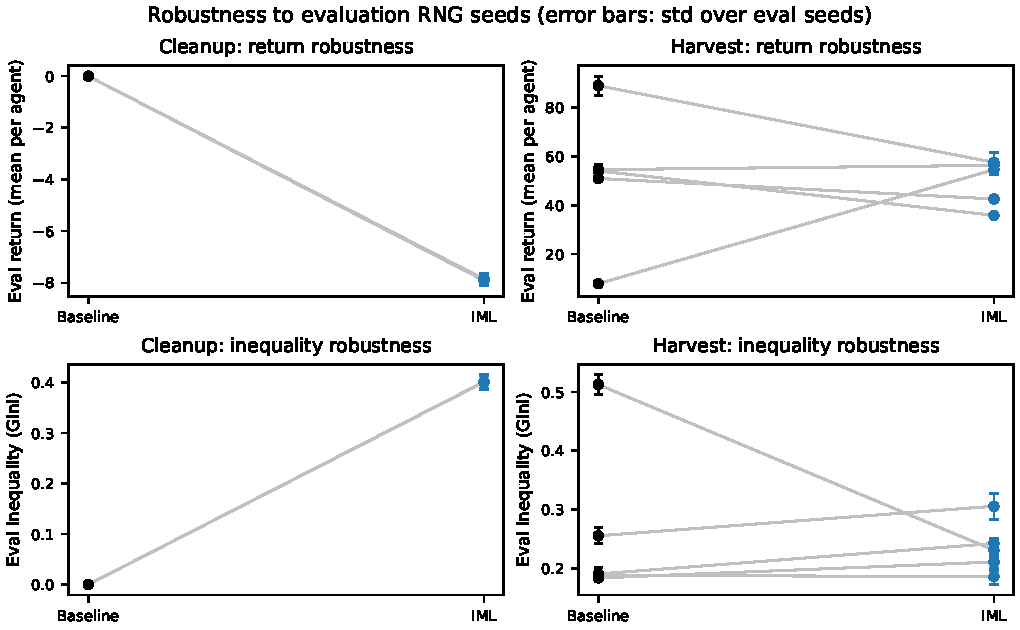
\includegraphics[width=0.75\linewidth]{figures/fig_eval_seed_robustness.pdf}
\caption{Robustness to evaluation RNG seeds. Each gray segment connects Baseline and IML means for a fixed \emph{training} seed; markers show per-policy means averaged over five evaluation seeds (50 episodes per seed), and error bars show the within-policy SD across evaluation seeds. Evaluation randomness is modest relative to effect sizes and (in \textsc{Harvest}) relative to training-seed variability.}
\label{fig:eval_seed_robustness}
\end{figure}

\section{Sensitivity to institutional false positives and review probability}
\label{app:sensitivity}

To isolate institutional parameter effects from learning dynamics, we perform an \emph{evaluation-only} sweep on \textsc{Cleanup} using trained IML checkpoints. We vary the per agent-step false-positive rate $p_{\mathrm{fp}}\in\{10^{-4},10^{-3},10^{-2}\}$ and the review probability $p_{\mathrm{review}}\in\{0,0.2,0.5,0.8\}$ while holding the learned policy fixed. Each sweep point averages 20 evaluation episodes (environment seed 0) for each training seed and is then averaged across the five training seeds. This protocol makes the welfare impact of enforcement error directly visible without confounding by policy adaptation.

Figure~\ref{fig:sensitivity_cleanup_iml} confirms two regularities relevant for deployable institutions. First, net sanction volume scales approximately linearly with $p_{\mathrm{fp}}$, consistent with the linear scaling $\mathbb{E}[\mathrm{FP}] \approx p_{\mathrm{fp}} \, N \, T$, producing a predictable ``sanction tax'' on welfare of approximately $-(\sigma/N)\,\mathbb{E}[\mathrm{net\ sanctions}]$. Second, increasing $p_{\mathrm{review}}$ reduces net sanctions and partially restores welfare by overturning a larger fraction of false detections. For example, reducing $p_{\mathrm{fp}}$ to $10^{-4}$ and increasing $p_{\mathrm{review}}$ to 0.8 yields near-zero welfare loss (mean return $\approx -0.02$) with negligible sanction overhead (net sanctions $\approx 0.3$ per episode). A review-capacity bottleneck can be approximated, to first order, as lower effective $p_{\mathrm{review}}$ together with larger settlement delay $D$. Our sweep varies only $p_{\mathrm{review}}$; because Section~\ref{sec:delay} shows that larger $D$ also weakens deterrence and prolongs wrongful burden, real queueing or institutional gridlock would generally shift these curves in an unfavorable direction. The overall implication is that deployable institutions require explicit \emph{error budgeting} and calibrated due process, particularly in long-horizon settings where per-step noise accumulates.

\begin{figure}[!ht]
\centering
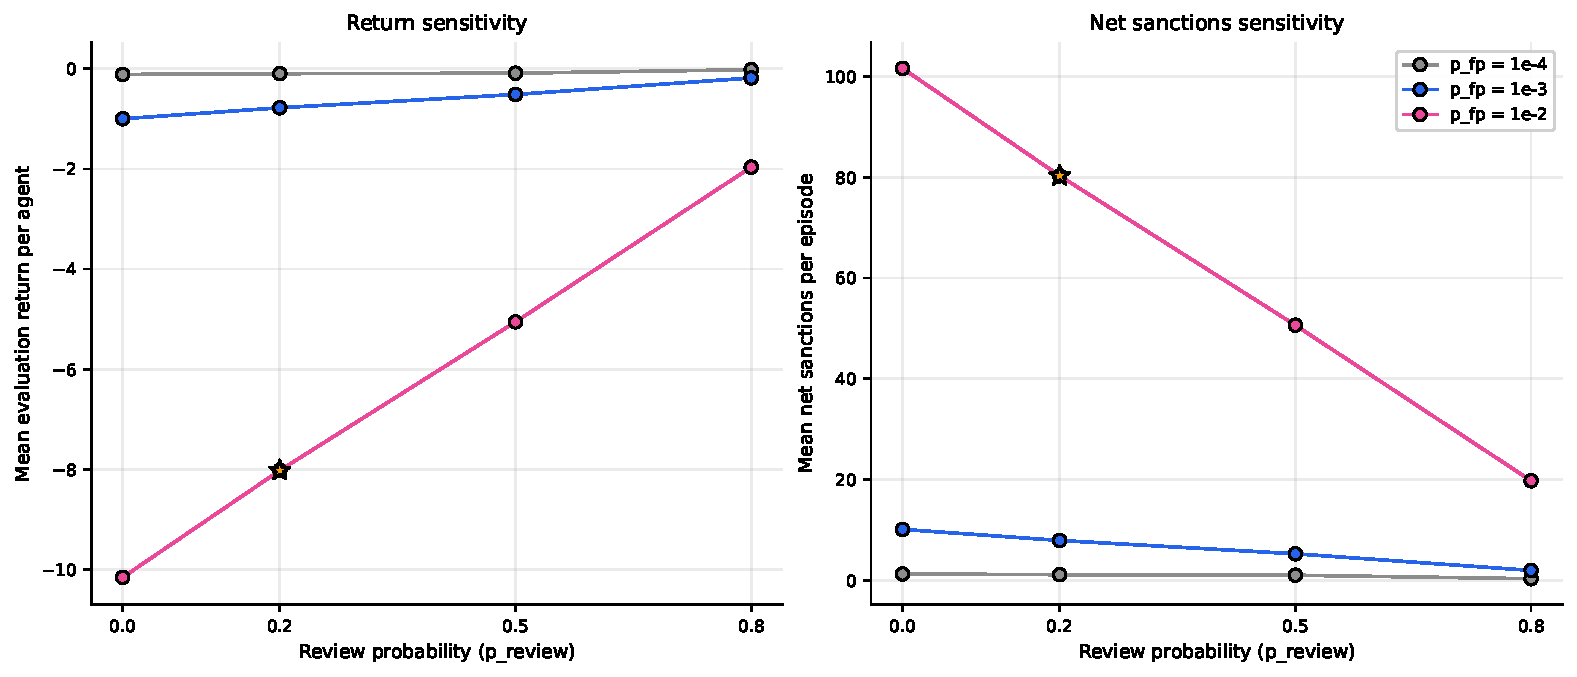
\includegraphics[width=0.75\linewidth]{figures/fig_sensitivity_cleanup_iml.pdf}
\caption{\textbf{Evaluation-only sensitivity of \textsc{Cleanup}--IML to institutional parameters.} We re-evaluate trained IML \textsc{Cleanup} policies while varying the per-step false-positive rate $p_{\mathrm{fp}}$ and review probability $p_{\mathrm{review}}$, holding policies fixed. Left: mean evaluation return per agent. Right: mean net sanctions per episode. Lines denote $p_{\mathrm{fp}}$ and the marker highlights the nominal configuration $(p_{\mathrm{fp}},p_{\mathrm{review}})=(10^{-2},0.2)$.}
\label{fig:sensitivity_cleanup_iml}
\end{figure}



%%%%%%%%%%%%%%%%%%%%%%%%%%%%%%%%%%%%%%%%%%
%\isPreprints{}{% This command is only used for ``preprints''.
\begin{adjustwidth}{-\extralength}{0cm}
%} % If the paper is ``preprints'', please uncomment this parenthesis.
%\printendnotes[custom] % Un-comment to print a list of endnotes

\reftitle{References}

% Please provide either the correct journal abbreviation (e.g. according to the “List of Title Word Abbreviations” http://www.issn.org/services/online-services/access-to-the-ltwa/) or the full name of the journal.
% Citations and References in Supplementary files are permitted provided that they also appear in the reference list here. 

%=====================================
% References, variant A: external bibliography
%=====================================
\bibliography{references}



% If authors have biography, please use the format below
%\section*{Short Biography of Authors}
%\bio
%{\raisebox{-0.35cm}{\includegraphics[width=3.5cm,height=5.3cm,clip,keepaspectratio]{Definitions/author1.pdf}}}
%{\textbf{Firstname Lastname} Biography of first author}
%
%\bio
%{\raisebox{-0.35cm}{\includegraphics[width=3.5cm,height=5.3cm,clip,keepaspectratio]{Definitions/author2.jpg}}}
%{\textbf{Firstname Lastname} Biography of second author}

% For the MDPI journals use author-date citation, please follow the formatting guidelines on http://www.mdpi.com/authors/references
% To cite two works by the same author: \citeauthor{ref-journal-1a} (\citeyear{ref-journal-1a}, \citeyear{ref-journal-1b}). This produces: Whittaker (1967, 1975)
% To cite two works by the same author with specific pages: \citeauthor{ref-journal-3a} (\citeyear{ref-journal-3a}, p. 328; \citeyear{ref-journal-3b}, p.475). This produces: Wong (1999, p. 328; 2000, p. 475)

%%%%%%%%%%%%%%%%%%%%%%%%%%%%%%%%%%%%%%%%%%
%% for journal Sci
%\reviewreports{\\
%Reviewer 1 comments and authors’ response\\
%Reviewer 2 comments and authors’ response\\
%Reviewer 3 comments and authors’ response
%}
%%%%%%%%%%%%%%%%%%%%%%%%%%%%%%%%%%%%%%%%%%
\PublishersNote{}
%\isPreprints{}{% This command is only used for ``preprints''.
\end{adjustwidth}
%} % If the paper is ``preprints'', please uncomment this parenthesis.
\end{document}

